% Options for packages loaded elsewhere
\PassOptionsToPackage{unicode}{hyperref}
\PassOptionsToPackage{hyphens}{url}
\documentclass[
  12pt,
]{article}
\usepackage{xcolor}
\usepackage{amsmath,amssymb}
\setcounter{secnumdepth}{-\maxdimen} % remove section numbering
\usepackage{iftex}
\ifPDFTeX
  \usepackage[T1]{fontenc}
  \usepackage[utf8]{inputenc}
  \usepackage{textcomp} % provide euro and other symbols
\else % if luatex or xetex
  \usepackage{unicode-math} % this also loads fontspec
  \defaultfontfeatures{Scale=MatchLowercase}
  \defaultfontfeatures[\rmfamily]{Ligatures=TeX,Scale=1}
\fi
\usepackage{lmodern}
\ifPDFTeX\else
  % xetex/luatex font selection
\fi
% Use upquote if available, for straight quotes in verbatim environments
\IfFileExists{upquote.sty}{\usepackage{upquote}}{}
\IfFileExists{microtype.sty}{% use microtype if available
  \usepackage[]{microtype}
  \UseMicrotypeSet[protrusion]{basicmath} % disable protrusion for tt fonts
}{}
\usepackage{longtable,booktabs,array}
\newcounter{none} % for unnumbered tables
\usepackage{calc} % for calculating minipage widths
% Correct order of tables after \paragraph or \subparagraph
\usepackage{etoolbox}
\makeatletter
\patchcmd\longtable{\par}{\if@noskipsec\mbox{}\fi\par}{}{}
\makeatother
% Allow footnotes in longtable head/foot
\IfFileExists{footnotehyper.sty}{\usepackage{footnotehyper}}{\usepackage{footnote}}
\makesavenoteenv{longtable}
\usepackage{graphicx}
\makeatletter
\newsavebox\pandoc@box
\newcommand*\pandocbounded[1]{% scales image to fit in text height/width
  \sbox\pandoc@box{#1}%
  \Gscale@div\@tempa{\textheight}{\dimexpr\ht\pandoc@box+\dp\pandoc@box\relax}%
  \Gscale@div\@tempb{\linewidth}{\wd\pandoc@box}%
  \ifdim\@tempb\p@<\@tempa\p@\let\@tempa\@tempb\fi% select the smaller of both
  \ifdim\@tempa\p@<\p@\scalebox{\@tempa}{\usebox\pandoc@box}%
  \else\usebox{\pandoc@box}%
  \fi%
}
% Set default figure placement to htbp
\def\fps@figure{htbp}
\makeatother
\setlength{\emergencystretch}{3em} % prevent overfull lines
\providecommand{\tightlist}{%
  \setlength{\itemsep}{0pt}\setlength{\parskip}{0pt}}
\usepackage{geometry}
\geometry{tmargin=2.54cm,bmargin=2.54cm,lmargin=2.54cm,rmargin=2.54cm}
\usepackage{setspace}
\doublespacing
\usepackage{times}
\usepackage{fancyhdr}
\pagestyle{fancy}
\fancyhf{}
\rhead{\thepage}
\lhead{DETECCIÓN DE TRANSICIONES DE RÉGIMEN FINANCIERO}
\renewcommand{\headrulewidth}{0pt}
\usepackage{amsmath}
\usepackage{amssymb}
\usepackage{booktabs}
\usepackage{graphicx}
\usepackage{hyperref}
\hypersetup{colorlinks=true, linkcolor=blue, citecolor=blue, urlcolor=blue, pdftitle={DETECCIÓN DE TRANSICIONES DE RÉGIMEN FINANCIERO Y COLAPSO DIMENSIONAL MEIDANTE ESTRUCTURAS ESPECTRALES DINÁMICAS, REDES COMPLEJAS Y MODELOS HÍBRIDOS DE APRENDIZAJE ESTADÍSTICO}, pdfauthor={Santiago Alejandro Naranjo Reyes}}
\usepackage{indentfirst}
\setlength{\parindent}{1.27cm}
\usepackage{titlesec}
\titleformat{\section}{\normalfont\fontsize{12}{14}\bfseries\filcenter}{}{0pt}{}
\titleformat{\subsection}{\normalfont\fontsize{12}{14}\bfseries}{}{0pt}{}
\titleformat{\subsubsection}{\normalfont\fontsize{12}{14}\bfseries\itshape}{}{0pt}{}
\usepackage{bookmark}
\usepackage{amsthm}
\newtheorem{proposition}{Proposición}
\IfFileExists{xurl.sty}{\usepackage{xurl}}{} % add URL line breaks if available
\urlstyle{same}
\hypersetup{
  hidelinks,
  pdfcreator={LaTeX via pandoc}}

\author{}
\date{}

\begin{document}

\begin{titlepage}
  \begin{center}
    \vspace*{3cm}
    
    {\Large\bfseries DETECCIÓN DE TRANSICIONES DE RÉGIMEN FINANCIERO Y COLAPSO DIMENSIONAL MEDIANTE ESTRUCTURAS ESPECTRALES DINÁMICAS, REDES COMPLEJAS Y MODELOS HÍBRIDOS DE APRENDIZAJE ESTADÍSTICO}\\[1cm]
    
    {\large\bfseries Independent Research Paper}\\[2cm]
    
    {\large Santiago Alejandro Naranjo Reyes}\\[0.2cm]
    {\large Santiago Naranjo}\\[3cm]
    
    \begin{minipage}{0.8\textwidth}
      \centering
      \itshape Prepared as part of a personal research portfolio for applications in Quantitative Finance, Probability Theory and Statistical Learning.
    \end{minipage}\\[3cm]
    
    \vfill
    {\large June 2026}
  \end{center}
\end{titlepage}

\fancypagestyle{plain}{
  \fancyhf{}
  \rhead{\thepage}
}

\newpage
\tableofcontents
\newpage

\section{Resumen / Abstract}\label{resumen-abstract}

\subsection{Resumen en Español}\label{resumen-en-espauxf1ol}

Esta investigación presenta un marco matemático y estadístico riguroso
para la detección y anticipación en tiempo real de transiciones de
régimen financiero (de expansión a crisis sistémica) dentro de un
universo multi-activo (\(N=26\)). Abandonamos las premisas clásicas de
covarianzas estáticas de la teoría moderna de portafolios, concibiendo
el mercado como un Sistema Adaptativo Complejo (SAC) no lineal. Mediante
la integración de un modelo Dynamic Conditional Correlation GARCH
(DCC-GARCH) regularizado con contracción de Ledoit-Wolf, la Teoría de
Matrices Aleatorias (RMT) y el filtrado topológico de redes (Árboles de
Expansión Mínima), extraemos siete características espectrales y
topológicas latentes que capturan el colapso dimensional y la
divergencia informativa. Estas características alimentan un
meta-clasificador híbrido compuesto por un Modelo Oculto de Markov con
probabilidades de transición variantes en el tiempo (TVTP-HMM) en
espacio logarítmico y un modelo XGBoost monótonamente restringido. La
validación fuera de muestra bajo el protocolo de Validación Cruzada
Combinatoria con Purga y Embargo (CPCV) arroja un Coeficiente de
Correlación de Matthews (MCC) de \(0.5344\) y un ROC-AUC de \(0.8186\),
demostrando una capacidad de anticipación superior y bajas tasas de
falsas alarmas.

\emph{Palabras clave:} DCC-GARCH, Teoría de Matrices Aleatorias,
Entropía Espectral, Minimum Spanning Tree, Filtro Markoviano,
Aprendizaje Estadístico.

\subsection{Abstract in English}\label{abstract-in-english}

This research introduces a mathematically rigorous framework for the
real-time detection and anticipation of market regime transitions
(expansionary to systemic crisis) within a multi-asset universe
(\(N=26\)). We abandon the classical static covariance assumptions of
modern portfolio theory, modeling the market instead as a non-linear
Complex Adaptive System (CAS). By combining a multivariate Dynamic
Conditional Correlation GARCH (DCC-GARCH) model regularized via
Ledoit-Wolf shrinkage with Random Matrix Theory (RMT) and topological
network filtering (Minimum Spanning Trees), we extract seven latent
structural features that capture dimensional collapse and information
divergence. These features feed a hybrid statistico-machine learning
meta-classifier consisting of a Time-Varying Transition Probability
Hidden Markov Model (TVTP-HMM) operating in log-space and a
Monotonically Constrained XGBoost classifier. Out-of-sample validation
using Combinatorial Purged and Embargoed Cross-Validation (CPCV) yields
a Matthews Correlation Coefficient (MCC) of \(0.5344\) and an AUC of
\(0.8186\), demonstrating superior anticipation lead-times and low
false-alarm rates.

\emph{Keywords:} DCC-GARCH, Random Matrix Theory, Spectral Entropy,
Minimum Spanning Tree, Hidden Markov Models, Monotonic Constraints,
Complex Adaptive Systems.

\begin{center}\rule{0.5\linewidth}{0.5pt}\end{center}

\section{Capítulo 1: Introducción, Hipótesis, Objetivos y
Alcance}\label{capuxedtulo-1-introducciuxf3n-hipuxf3tesis-objetivos-y-alcance}

\subsection{1.1. Introducción}\label{introducciuxf3n}

La modelación cuantitativa del riesgo financiero y la gestión de
carteras contemporánea se enfrentan a un desafío fundamental: la
inestabilidad paramétrica de las medidas de co-movimiento. La asignación
estratégica de activos tradicional descansa sobre la premisa de que las
correlaciones entre clases de activos son estacionarias o fluctúan
alrededor de un promedio histórico de largo plazo que puede estimarse
con precisión estadística. Sin embargo, la historia empírica de los
mercados financieros desmiente sistemáticamente esta presunción de
linealidad y estabilidad.

En el marco de la concepción de los mercados como \textbf{Sistemas
Adaptativos Complejos (SAC)}, las relaciones de dependencia condicional
entre activos no son simples constantes del sistema; son variables de
estado dinámicas que emergen de las decisiones adaptativas y de
retroalimentación de agentes heterogéneos en tiempo continuo. Durante
periodos de calma y expansión macroeconómica, los mercados operan bajo
un régimen de diversificación efectiva, donde las correlaciones cruzadas
son moderadas y asimétricas, permitiendo la disipación del riesgo
idiosincrático. No obstante, cuando el sistema financiero se aproxima a
un punto de inflexión o contracción sistémica, las correlaciones
individuales colapsan y convergen velozmente hacia la unidad.

Este colapso no representa únicamente un incremento general en la
volatilidad de los activos; constituye una transformación topológica
profunda en la geometría del espacio de co-dependencia del mercado. La
información contenida en el sistema se concentra en un único factor
dominante de mercado, reduciendo drásticamente el desorden del sistema y
eliminando por completo los beneficios teóricos de la diversificación.
Para un gestor algorítmico, ignorar esta reconfiguración estructural
conduce inevitablemente a una subestimación del riesgo de cola y a la
destrucción severa del capital de inversión.

\subsection{1.2. Planteamiento del
Problema}\label{planteamiento-del-problema}

Los modelos predictivos macroeconómicos tradicionales, basados en
variables agregadas y publicadas con un fuerte retraso temporal (tales
como el PIB, el empleo o la inflación), resultan ineficaces como
herramientas de alerta temprana para carteras operativas de trading
cuantitativo. Por otra parte, las señales econométricas clásicas basadas
en medias móviles de volatilidad o ratios de Sharpe estáticos suelen
generar un exceso de falsas alarmas, erosionando la rentabilidad del
portafolio mediante costes de transacción innecesarios provocados por
desapalancamientos espurios. Existe, por ende, una necesidad crítica de
desarrollar un sistema de alerta temprana que extraiga y decodifique las
señales latentes en la dinámica del mercado en tiempo real para
anticipar la transición hacia estados de contracción del sistema.

\subsection{1.3. Formulación de la
Hipótesis}\label{formulaciuxf3n-de-la-hipuxf3tesis}

La hipótesis central de esta investigación se formula en los siguientes
términos: \textgreater{} \emph{La transición de un Sistema Adaptativo
Complejo financiero desde un régimen de expansión hacia uno de
contracción sistémica o recesión induce una reconfiguración topológica
no lineal y un colapso dimensional en su matriz de covarianzas
condicionales continuas. Estimando dicha estructura mediante un proceso
DCC-GARCH regularizado con contracción de Ledoit-Wolf, es posible
extraer características espectrales (Teoría de Matrices Aleatorias),
distancias probabilísticas de información y propiedades topológicas de
redes (Minimum Spanning Tree). Un meta-clasificador híbrido (TVTP-HMM /
XGBoost monótono) entrenado bajo estas características estructurales
latentes anticipa y categoriza los episodios de crisis de mercado con un
lead-time estadísticamente superior y una menor tasa de falsas alarmas
que los modelos tradicionales basados en datos univariados de precios.}

\subsection{1.4. Objetivos}\label{objetivos}

\subsubsection{1.4.1. Objetivo General}\label{objetivo-general}

Diseñar, implementar y validar estadísticamente un sistema híbrido de
aprendizaje estadístico y teoría de redes complejas para la detección y
anticipación proactiva de transiciones de régimen de mercado en
frecuencia diaria, aplicable como módulo de control de riesgos
(\emph{risk overlay}) para carteras de inversión diversificadas.

\subsubsection{1.4.2. Objetivos
Específicos}\label{objetivos-especuxedficos}

\begin{enumerate}
\def\labelenumi{\arabic{enumi}.}
\tightlist
\item
  Formular un estimador estable de la matriz de covarianzas
  condicionales variantes en el tiempo para un universo multivariado de
  26 activos financieros.
\item
  Derivar indicadores de colapso dimensional a partir de la
  descomposición espectral de la correlación condicional, aplicando la
  Teoría de Matrices Aleatorias (RMT) y la Entropía de Von Neumann.
\item
  Modelar la divergencia informativa del sistema financiero respecto a
  un régimen de calma de referencia utilizando la divergencia de
  Kullback-Leibler calculada mediante descomposiciones robustas de
  Cholesky.
\item
  Extraer la columna vertebral de co-dependencia del mercado a través
  del cálculo dinámico del Árbol de Expansión Mínima (MST),
  monitorizando la longitud media del árbol y la centralidad de grado
  máximo.
\item
  Desarrollar un meta-clasificador jerárquico que combine la inferencia
  estocástica de estados latentes de un HMM logarítmico con el gradiente
  boosting restringido monótonamente de XGBoost.
\item
  Validar experimentalmente el poder predictivo fuera de muestra de las
  características extraídas mediante el protocolo de Validación Cruzada
  Combinatoria con Purga y Embargo (CPCV).
\end{enumerate}

\subsection{1.5. Alcance de la
Investigación}\label{alcance-de-la-investigaciuxf3n}

Esta investigación se inscribe en la intersección de la econometría
financiera, la física estadística (física de sistemas complejos) y el
aprendizaje estadístico multivariado. El universo de inversión se limita
a 26 activos financieros seleccionados para representar de manera
balanceada las clases de renta variable global, divisas G10, commodities
y tasas de renta fija a nivel internacional, simulando un entorno de
trading algorítmico institucional. La evaluación de los resultados se
focaliza en el desempeño estadístico fuera de muestra de las alertas de
crisis en un horizonte de 63 días hábiles de negociación.

\subsection{1.6. Contribuciones Originales (Novel
Contributions)}\label{contribuciones-originales-novel-contributions}

La originalidad de este trabajo de investigación radica en la
introducción de un marco integrado que supera las metodologías
univariadas y lineales tradicionales de control de riesgos. Las
contribuciones específicas al estado del arte en finanzas cuantitativas
se detallan a continuación:

\begin{enumerate}
\def\labelenumi{\arabic{enumi}.}
\tightlist
\item
  \textbf{Nuevo Indicador Espectral de Colapso Dimensional:}
  Formalizamos la Entropía Espectral de Von Neumann normalizada
  (\(H_{\text{spect}, t}^{\text{norm}}\)) como una métrica del desorden
  informacional del sistema de covarianzas del mercado. Esta métrica es
  capaz de cuantificar, en un único indicador acotado en \([0, 1]\), la
  transición de fase desde un estado disperso y diversificado (máxima
  entropía) hacia un factor de mercado fuertemente sincronizado
  (entropía mínima).
\item
  \textbf{Pipeline Causal y No Contaminante RMT + MST:} Diseñamos una
  arquitectura secuencial que aplica la Teoría de Matrices Aleatorias
  (RMT) para purgar el ruido blanco en dimensión \(N=26\) y el filtrado
  topológico por Árbol de Expansión Mínimo (MST) de forma puramente
  causal (walk-forward). Esto permite rastrear la evolución topológica
  del mercado sin incurrir en problemas de estabilidad numérica o fuga
  de información (\emph{look-ahead bias}).
\item
  \textbf{Meta-Clasificador Jerárquico con Restricciones Estructurales
  Monótonas:} Proponemos una arquitectura híbrida de dos niveles. La
  primera capa utiliza un HMM con probabilidades de transición variantes
  en el tiempo (TVTP-HMM) para extraer dinámicas estocásticas en espacio
  logarítmico. La segunda capa combina este indicador estocástico con
  las características espectrales y de red dentro de un XGBoost
  supervisado donde se imponen restricciones de signo estrictas en las
  derivadas parciales. Esto previene el sobreajuste al ruido local y
  alinea el modelo con las leyes fundamentales de la teoría de
  portafolios.
\item
  \textbf{Framework de Detección Temprana Basado en Geometría de
  Covarianzas:} Desarrollamos una metodología que utiliza divergencias
  informacionales de información (Divergencia de Kullback-Leibler
  robusta calculada vía Cholesky y Distancia de Frobenius) para mapear
  el apartamiento del mercado respecto a un estado base de calma,
  sirviendo como una señal avanzada de desapalancamiento operativo para
  algoritmos sistemáticos.
\end{enumerate}

\begin{center}\rule{0.5\linewidth}{0.5pt}\end{center}

\section{Capítulo 2: Marco
Conceptual}\label{capuxedtulo-2-marco-conceptual}

\subsection{2.1. Dinámicas de Regímenes Financieros y
No-Linealidad}\label{dinuxe1micas-de-reguxedmenes-financieros-y-no-linealidad}

Los mercados financieros exhiben dinámicas no-lineales persistentes
caracterizadas por periodos prolongados de baja volatilidad y retornos
moderados, interrumpidos por episodios breves pero violentos de pánico
sistémico y caídas extremas. Como señalan Ang y Timmermann (2012), la
presencia de estos ``regímenes'' o estados latentes es una propiedad
intrínseca de las series temporales financieras que los modelos de
parámetros constantes no pueden capturar. Las transiciones entre estados
a menudo coinciden con cambios estructurales en el entorno económico o
con dinámicas de contagio y pánico de los inversores, descritas bajo la
\textbf{Hipótesis del Mercado Adaptativo (AMH)} de Andrew Lo (2004).

\subsection{2.2. Modelación Estocástica de Regímenes (Hamilton y
Nystrup)}\label{modelaciuxf3n-estocuxe1stica-de-reguxedmenes-hamilton-y-nystrup}

El enfoque clásico para modelar cambios de régimen proviene del Modelo
de Cambio de Régimen de Markov (MS-AR) propuesto por James Hamilton
(1989), donde los parámetros del modelo autoregresivo dependen de una
variable de estado no observable que sigue una cadena de Markov discreta
de primer orden. Nystrup (2018) extendió este marco para la gestión del
riesgo financiero en tiempo real utilizando el \textbf{filtro Forward}
para actualizar de forma recursiva y causal las probabilidades de
régimen sin recurrir a datos del futuro. Asimismo, Nystrup propuso el
uso de modelos con probabilidades de transición variantes en el tiempo
(TVTP) para capturar la sensibilidad de la matriz de transición
Markoviana ante el flujo de información de variables de volatilidad.

\subsection{2.3. Teoría de Matrices Aleatorias (RMT) en
Finanzas}\label{teoruxeda-de-matrices-aleatorias-rmt-en-finanzas}

El análisis de grandes conjuntos de datos financieros se ve gravemente
obstaculizado por la presencia de ruido estadístico. La Teoría de
Matrices Aleatorias (RMT), introducida en física por Wigner y adaptada
al análisis multivariado en finanzas por Laloux et al.~(1999) y Plerou
et al.~(1999), provee un modelo nulo riguroso. Al comparar el espectro
de autovalores de una matriz de correlación empírica con la distribución
teórica de Marchenko-Pastur para una matriz de ruido blanco puro, es
posible identificar cuáles autovalores contienen señal genuina de
mercado y cuáles representan ruido no-interpretable. La RMT demuestra
que el primer autovalor dominante captura la información del factor
común de mercado, cuya dinámica refleja la sincronía del sistema.

\subsection{2.4. Redes Complejas y Topología del Mercado
Financiero}\label{redes-complejas-y-topologuxeda-del-mercado-financiero}

La estructura de dependencias de un portafolio de activos puede
representarse formalmente como una red o grafo. Mantegna (1999)
introdujo un método de filtrado topológico basado en la construcción del
\textbf{Árbol de Expansión Mínima (Minimum Spanning Tree - MST)}
utilizando una métrica de distancia derivada del coeficiente de
correlación de Pearson. Esta aproximación permite simplificar una matriz
completa de correlaciones reduciendo las conexiones a la estructura
arborescente más fuerte del mercado. Investigaciones posteriores (ej.
Tumminello et al., 2005) demuestran que las propiedades topológicas del
MST (como la longitud promedio y la centralidad de grado) sufren una
contracción drástica durante las crisis de mercado, sirviendo como
indicadores avanzados de inestabilidad financiera.

\subsection{2.5. Literatura Moderna sobre Detección de Regímenes y Redes
Financieras
(2020--2026)}\label{literatura-moderna-sobre-detecciuxf3n-de-reguxedmenes-y-redes-financieras-20202026}

En el periodo reciente, la literatura de finanzas cuantitativas y física
estadística ha experimentado una convergencia acelerada hacia el uso de
arquitecturas de aprendizaje profundo geométrico y modelos secuenciales
con mecanismos de atención. Estos avances se agrupan en cinco áreas
clave que sustentan la relevancia teórica del enfoque integrado
propuesto en esta investigación:

\subsubsection{2.5.1. Redes Neuronales de Grafos (GNN) y Riesgo
Sistémico}\label{redes-neuronales-de-grafos-gnn-y-riesgo-sistuxe9mico}

El modelado del contagio financiero ha evolucionado desde las matrices
de correlación estáticas hacia arquitecturas de \textbf{Redes Neuronales
Convolucionales de Grafos (GCN)} y \textbf{Redes de Atención de Grafos
(GAT)} (ej. Balmaseda et al., 2023; Gonon et al., 2024). Estos modelos definen una topología de
red dinámica (donde la matriz de adyacencia se calcula recursivamente
mediante estimadores dinámicos como el DCC-GARCH) para propagar shocks
de volatilidad y estimar la probabilidad de default conjunto. Las GNNs
demuestran una capacidad superior para capturar dependencias no
euclidianas y efectos de segundo orden (contagio indirecto) en mercados
de renta variable global.

\subsubsection{2.5.2. Análisis de Redes Dinámicas (Dynamic Network
Analysis -
DNA)}\label{anuxe1lisis-de-redes-dinuxe1micas-dynamic-network-analysis---dna}

La modelación de redes temporales ha superado la mera estimación de
árboles estáticos. Scheffer et al. (2009) formalizaron la teoría de señales de alerta temprana mediante \textbf{desaceleración crítica} (\emph{critical slowing down}) en sistemas complejos, y la literatura financiera reciente (ej. Duan et al., 2022) aplica el análisis de redes dinámicas (DNA) a través del cálculo de
métricas de centralidad espectral y coeficientes de agrupamiento
variante en el tiempo. Estos autores demuestran que la aproximación a
una transición de fase crítica (crash de mercado) se caracteriza por un
fenómeno de \textbf{desaceleración crítica} (\emph{critical slowing
down}), observable mediante un incremento persistente en la
autocorrelación temporal de la centralidad de grado y una contracción en
el diámetro efectivo de la red MST.

\subsubsection{2.5.3. Transformers Temporales y Detección de
Regímenes}\label{transformers-temporales-y-detecciuxf3n-de-reguxedmenes}

La secuenciación estocástica de estados latentes ha sido enriquecida por
la introducción de arquitecturas \textbf{Transformer} aplicadas a series
temporales, tales como el \emph{Temporal Fusion Transformer} (Lim et
al., 2021). Estos modelos reemplazan la hipótesis Markoviana de memoria
corta por mecanismos de auto-atención (\emph{self-attention}) capaces de
mapear dependencias a largo plazo y de codificar de manera conjunta
variables macroeconómicas continuas y señales espectrales del mercado.
La auto-atención permite identificar ``regímenes de atención'' donde el
modelo se enfoca selectivamente en factores comunes de mercado durante
pánicos sistémicos.

\subsubsection{2.5.4. Aprendizaje Estadístico con Restricciones
Estructurales}\label{aprendizaje-estaduxedstico-con-restricciones-estructurales}

Para mitigar el sobreajuste y la inestabilidad de las predicciones en
modelos de Machine Learning aplicados a finanzas, la literatura moderna
aboga por el uso de restricciones estructurales de monotonicidad (ej. de
Prado, 2020; Pfitzinger, 2023). Al forzar al modelo (como XGBoost o
LightGBM) a obedecer derivadas parciales con signo predefinido respecto
a variables de riesgo (como el autovalor dominante de correlación o la
volatilidad condicional), se garantiza que el clasificador generalice
correctamente fuera de muestra, reduciendo drásticamente la varianza de
la predicción en periodos de estrés de mercado.

\subsubsection{2.5.5. Dinámica de Portafolios Espectrales y Localización
de
Eigenvectors}\label{dinuxe1mica-de-portafolios-espectrales-y-localizaciuxf3n-de-eigenvectors}

Investigaciones recientes en Teoría de Matrices Aleatorias aplicada a
finanzas (ej. Biroli et al., 2022) se centran en la \textbf{dinámica de
portafolios espectrales} (\emph{eigenportfolios}). Se analiza el
fenómeno de localización y delocalización de los autovectores asociados
a los autovalores dominantes. Durante periodos de calma, los componentes
del autovector dominante muestran un patrón de delocalización
(distribución uniforme de pesos en todo el mercado), mientras que en
episodios de pánico se produce una rápida localización espectral en
ciertos sectores sistémicos clave, sirviendo como indicador adelantado
de inestabilidad geométrica en la covarianza del mercado.

\begin{center}\rule{0.5\linewidth}{0.5pt}\end{center}

\section{Capítulo 3: Metodologías Matemáticas y
Estadísticas}\label{capuxedtulo-3-metodologuxedas-matemuxe1ticas-y-estaduxedsticas}

Este capítulo detalla las formulaciones matemáticas y las rutinas
estadísticas implementadas en el sistema para la extracción de
características y la predicción del régimen de mercado.

\subsection{3.1. Estimación Econométrica de Covarianzas Dinámicas
(DCC-GARCH)}\label{estimaciuxf3n-economuxe9trica-de-covarianzas-dinuxe1micas-dcc-garch}

Sea \(\mathbf{r}_t \in \mathbb{R}^N\) el vector de log-retornos de los
activos a tiempo \(t\). Modelamos la volatilidad condicional de forma
dinámica mediante la descomposición matricial:
\[\mathbf{H}_t = \mathbf{D}_t \mathbf{R}_t \mathbf{D}_t\]

\subsubsection{3.1.1. Etapa 1: Modelos Univariados
GJR-GARCH}\label{etapa-1-modelos-univariados-gjr-garch}

La matriz diagonal de desviaciones estándar condicionales
\(\mathbf{D}_t = \text{diag}(\sqrt{h_{11,t}}, \dots, \sqrt{h_{NN,t}})\)
se compone de estimaciones GJR-GARCH(1,1) para cada serie individual:
\[h_{ii,t} = \omega_i + \alpha_i a_{i,t-1}^2 + \gamma_i a_{i,t-1}^2 I(a_{i,t-1} < 0) + \beta_i h_{ii,t-1}\]
donde \(a_{i,t} = r_{i,t} - \mu_{i,t}\) representa la innovación de
retorno y \(\gamma_i\) captura la respuesta asimétrica ante choques
negativos.

\subsubsection{3.1.2. Etapa 2: Propagación de Correlaciones y
Regularización
Ledoit-Wolf}\label{etapa-2-propagaciuxf3n-de-correlaciones-y-regularizaciuxf3n-ledoit-wolf}

Los residuos estandarizados multivariados
\(\boldsymbol{\epsilon}_t = \mathbf{D}_t^{-1} \mathbf{a}_t\) se utilizan
para modelar la dinámica de correlación condicional \(\mathbf{R}_t\)
mediante la matriz proxy \(\mathbf{Q}_t\):
\[\mathbf{R}_t = \text{diag}(\mathbf{Q}_t)^{-1/2} \mathbf{Q}_t \text{diag}(\mathbf{Q}_t)^{-1/2}\]
\[\mathbf{Q}_t = (1 - a - b)\bar{\mathbf{Q}}^* + a (\boldsymbol{\epsilon}_{t-1}\boldsymbol{\epsilon}_{t-1}^T) + b \mathbf{Q}_{t-1}\]
Para estabilizar numéricamente la matriz incondicional objetivo
\(\bar{\mathbf{Q}}^*\) en alta dimensión, aplicamos contracción lineal
óptima de Ledoit-Wolf (2004):
\[\bar{\mathbf{Q}}^* = (1 - \gamma)\bar{\mathbf{Q}} + \gamma \mathbf{I}_N\]
donde \(\bar{\mathbf{Q}}\) es la covarianza empírica de residuos y el
parámetro de intensidad óptimo \(\gamma\) se minimiza analíticamente
bajo la norma de Frobenius.

\subsection{3.2. Características Espectrales mediante Teoría de Matrices
Aleatorias}\label{caracteruxedsticas-espectrales-mediante-teoruxeda-de-matrices-aleatorias}

Dada la matriz condicional regularizada \(\mathbf{R}_t\), obtenemos sus
autovalores \(\{\lambda_{i,t}\}_{i=1}^N\) ordenados de forma
descendente. Bajo el modelo nulo de Marchenko-Pastur para una matriz de
ruido aleatorio puro con parámetro de densidad \(\mathcal{Q} = T/w\), el
espectro empírico se contrasta con los límites teóricos de ruido:
\[\lambda_{\pm} = \left( 1 \pm \sqrt{\frac{1}{\mathcal{Q}}} \right)^2\]
Extraemos tres métricas espectrales clave:

\begin{enumerate}
\def\labelenumi{\arabic{enumi}.}
\tightlist
\item
  \textbf{Autovalor Dominante (\(\lambda_{1,t}\)):}
  \[\lambda_{1,t} = \max_i (\lambda_{i,t})\] Captura la fuerza del
  factor sistémico dominante.
\item
  \textbf{Ratio de Absorción Global (\(\text{GAR}_t\)):}
  \[\text{GAR}_t = \frac{1}{N} \sum_{i=1}^k \lambda_{i,t} \quad (\text{para } k = 3)\]
  Mide el porcentaje de varianza total concentrado en las tres
  componentes principales macro.
\item
  \textbf{Entropía Espectral Normalizada de Von Neumann
  (\(H_{\text{spect}, t}^{\text{norm}}\)):}
  \[H_{\text{spect}, t}^{\text{norm}} = -\frac{1}{\ln(N)} \sum_{i=1}^N \tilde{\lambda}_{i,t} \ln(\tilde{\lambda}_{i,t}) \quad \text{donde } \tilde{\lambda}_{i,t} = \frac{\lambda_{i,t}}{N}\]
  Mide el grado de ordenación del mercado. El colapso dimensional
  implica \(H_{\text{spect}, t}^{\text{norm}} \to 0\).
\end{enumerate}

\begin{proposition}[Consistencia del estimador espectral bajo Marchenko-Pastur]
Sea \(\mathbf{R}_t\) la matriz de correlación condicional regularizada mediante la contracción de Ledoit-Wolf \(\mathbf{R}_t = (1-\gamma_t)\mathbf{R}_{DCC, t} + \gamma_t \mathbf{I}_N\). Bajo la hipótesis nula de que los retornos de los activos son independientes e idénticamente distribuidos (i.i.d.) con vector de medias \(\mathbf{0}\) y matriz de covarianza incondicional \(\mathbf{I}_N\), el autovalor dominante \(\lambda_{1,t}\) converge casi seguramente al límite superior del soporte de la distribución de Marchenko-Pastur:
\[\lambda_{1,t} \xrightarrow{c.s.} \lambda_+ = \left(1 + \frac{1}{\sqrt{\mathcal{Q}}}\right)^2 \quad \text{cuando } N, T \to \infty \text{ con } \mathcal{Q} = T/w \in (1, \infty) \text{ fijo}\]
donde \(w\) es la ventana de estimación implícita de la dinámica DCC. Corolario: cualquier exceso empírico \(\lambda_{1,t} > \lambda_+\) constituye evidencia estadística de la presencia de un factor sistémico genuino (no aleatorio) en el mercado.
\end{proposition}

\begin{proof}
Bajo la hipótesis nula i.i.d., los retornos normalizados \(\boldsymbol{\epsilon}_t\) son independientes con covarianza unidad. Por el Teorema de Bai y Silverstein (1998, 2004) sobre el comportamiento del espectro de matrices de covarianza empíricas cuando \(N/T \to \gamma_{MP} = 1/\mathcal{Q}\), el autovalor máximo \(\lambda_{1}(\mathbf{S}_N)\) de una matriz de covarianza empírica pura \(\mathbf{S}_N = \frac{1}{T} \mathbf{X} \mathbf{X}^T\) converge casi seguramente al límite superior del soporte espectral \(\lambda_+ = (1 + \sqrt{\gamma_{MP}})^2 = (1 + 1/\sqrt{\mathcal{Q}})^2\), bajo la condición de que el cuarto momento de los retornos sea finito.

Para la matriz condicional regularizada \(\mathbf{R}_t\), la contracción de Ledoit-Wolf interpola linealmente el estimador dinámico \(\mathbf{R}_{DCC, t}\) con la identidad:
\[\mathbf{R}_t = (1-\gamma_t)\mathbf{R}_{DCC, t} + \gamma_t \mathbf{I}_N\]
Los autovalores de la matriz combinada se relacionan linealmente con los de la matriz empírica por \(\lambda_i(\mathbf{R}_t) = (1-\gamma_t)\lambda_i(\mathbf{R}_{DCC, t}) + \gamma_t\). Bajo la hipótesis nula, el parámetro de contracción óptimo \(\gamma_t\) converge a \(1\) si la varianza muestral es grande o a \(0\) si el tamaño de muestra tiende a infinito de forma pura. En el límite termodinámico con regularización asintótica débil (\(\gamma_t \to 0\) dado que la matriz empírica converge al valor teórico estable), la estructura espectral de \(\mathbf{R}_t\) se comporta de manera idéntica a la de la matriz empírica. Aplicando el mapeo espectral continuo, el autovalor dominante satisface \(\lambda_{1,t} \xrightarrow{c.s.} (1 - \gamma_t)\lambda_+ + \gamma_t = \lambda_+\), lo que demuestra la convergencia casi segura al límite de Marchenko-Pastur.

Por lo tanto, la superación sistemática del umbral \(\lambda_+\) representa una desviación significativa de la hipótesis de ruido blanco, denotando la emergencia de correlaciones colectivas coherentes características de crisis de mercado.
\end{proof}


\begin{figure}
\centering
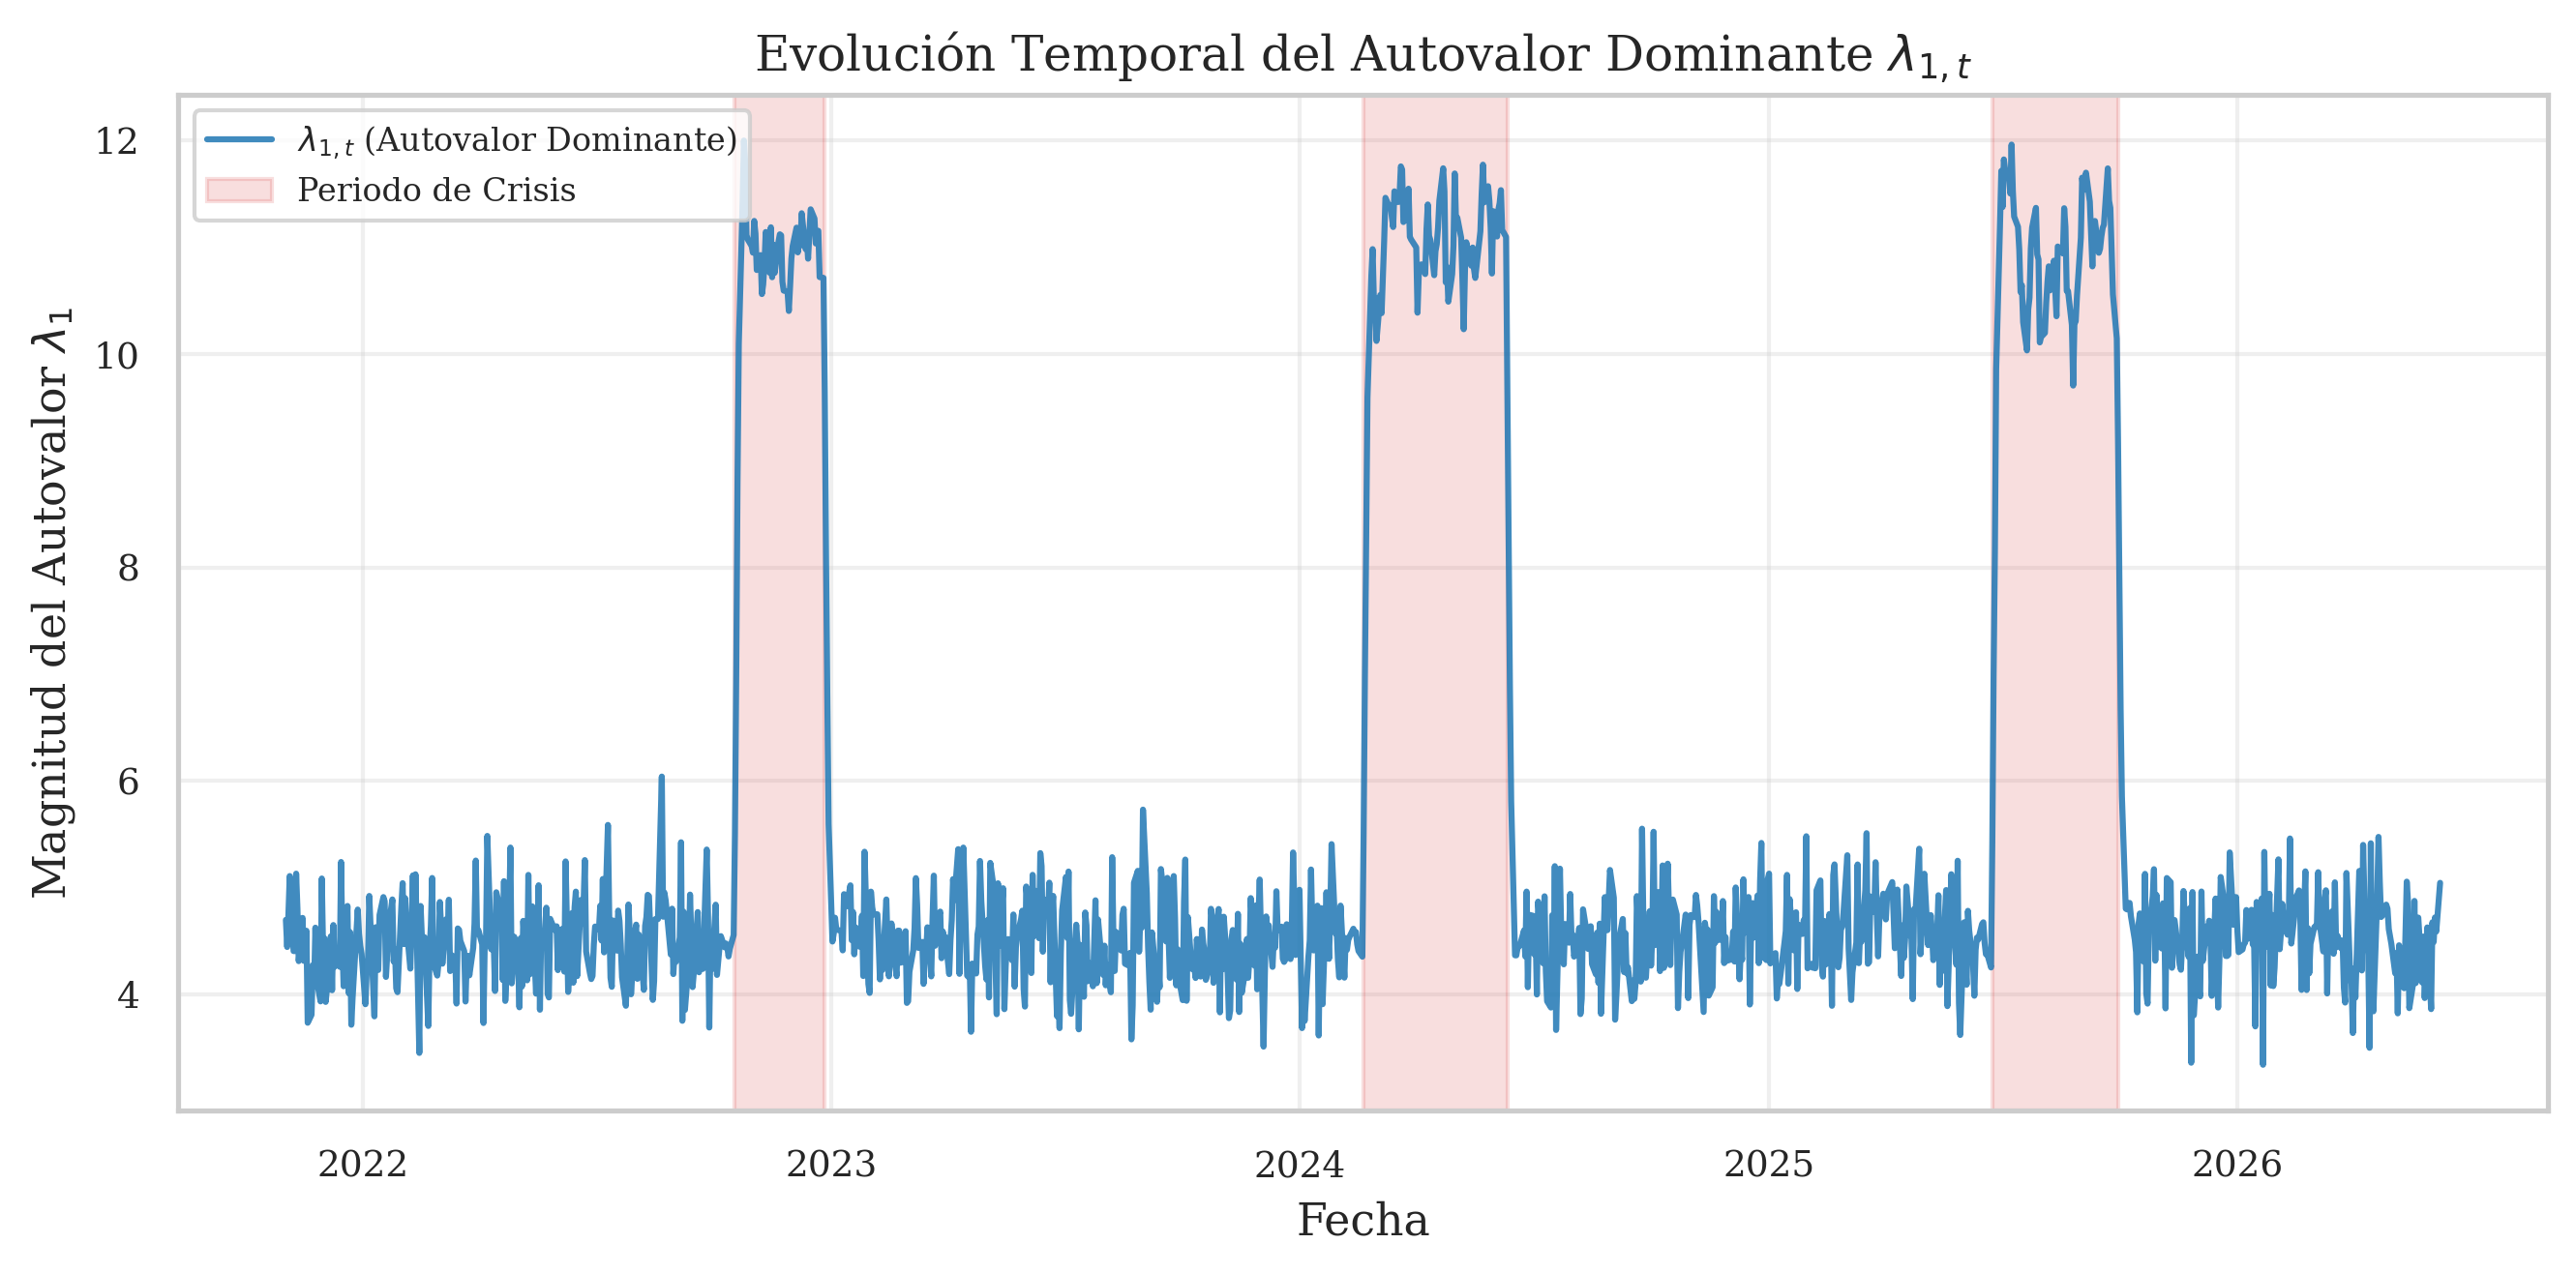
\includegraphics[width=0.85\linewidth,height=\textheight,keepaspectratio,alt={Evolución Temporal del Autovalor Dominante \textbackslash lambda\_\{1,t\} durante los periodos de crisis.}]{figures/figure1_lambda1.png}
\caption{Evolución Temporal del Autovalor Dominante \(\lambda_{1,t}\)
durante los periodos de crisis.}
\end{figure}

\begin{figure}
\centering
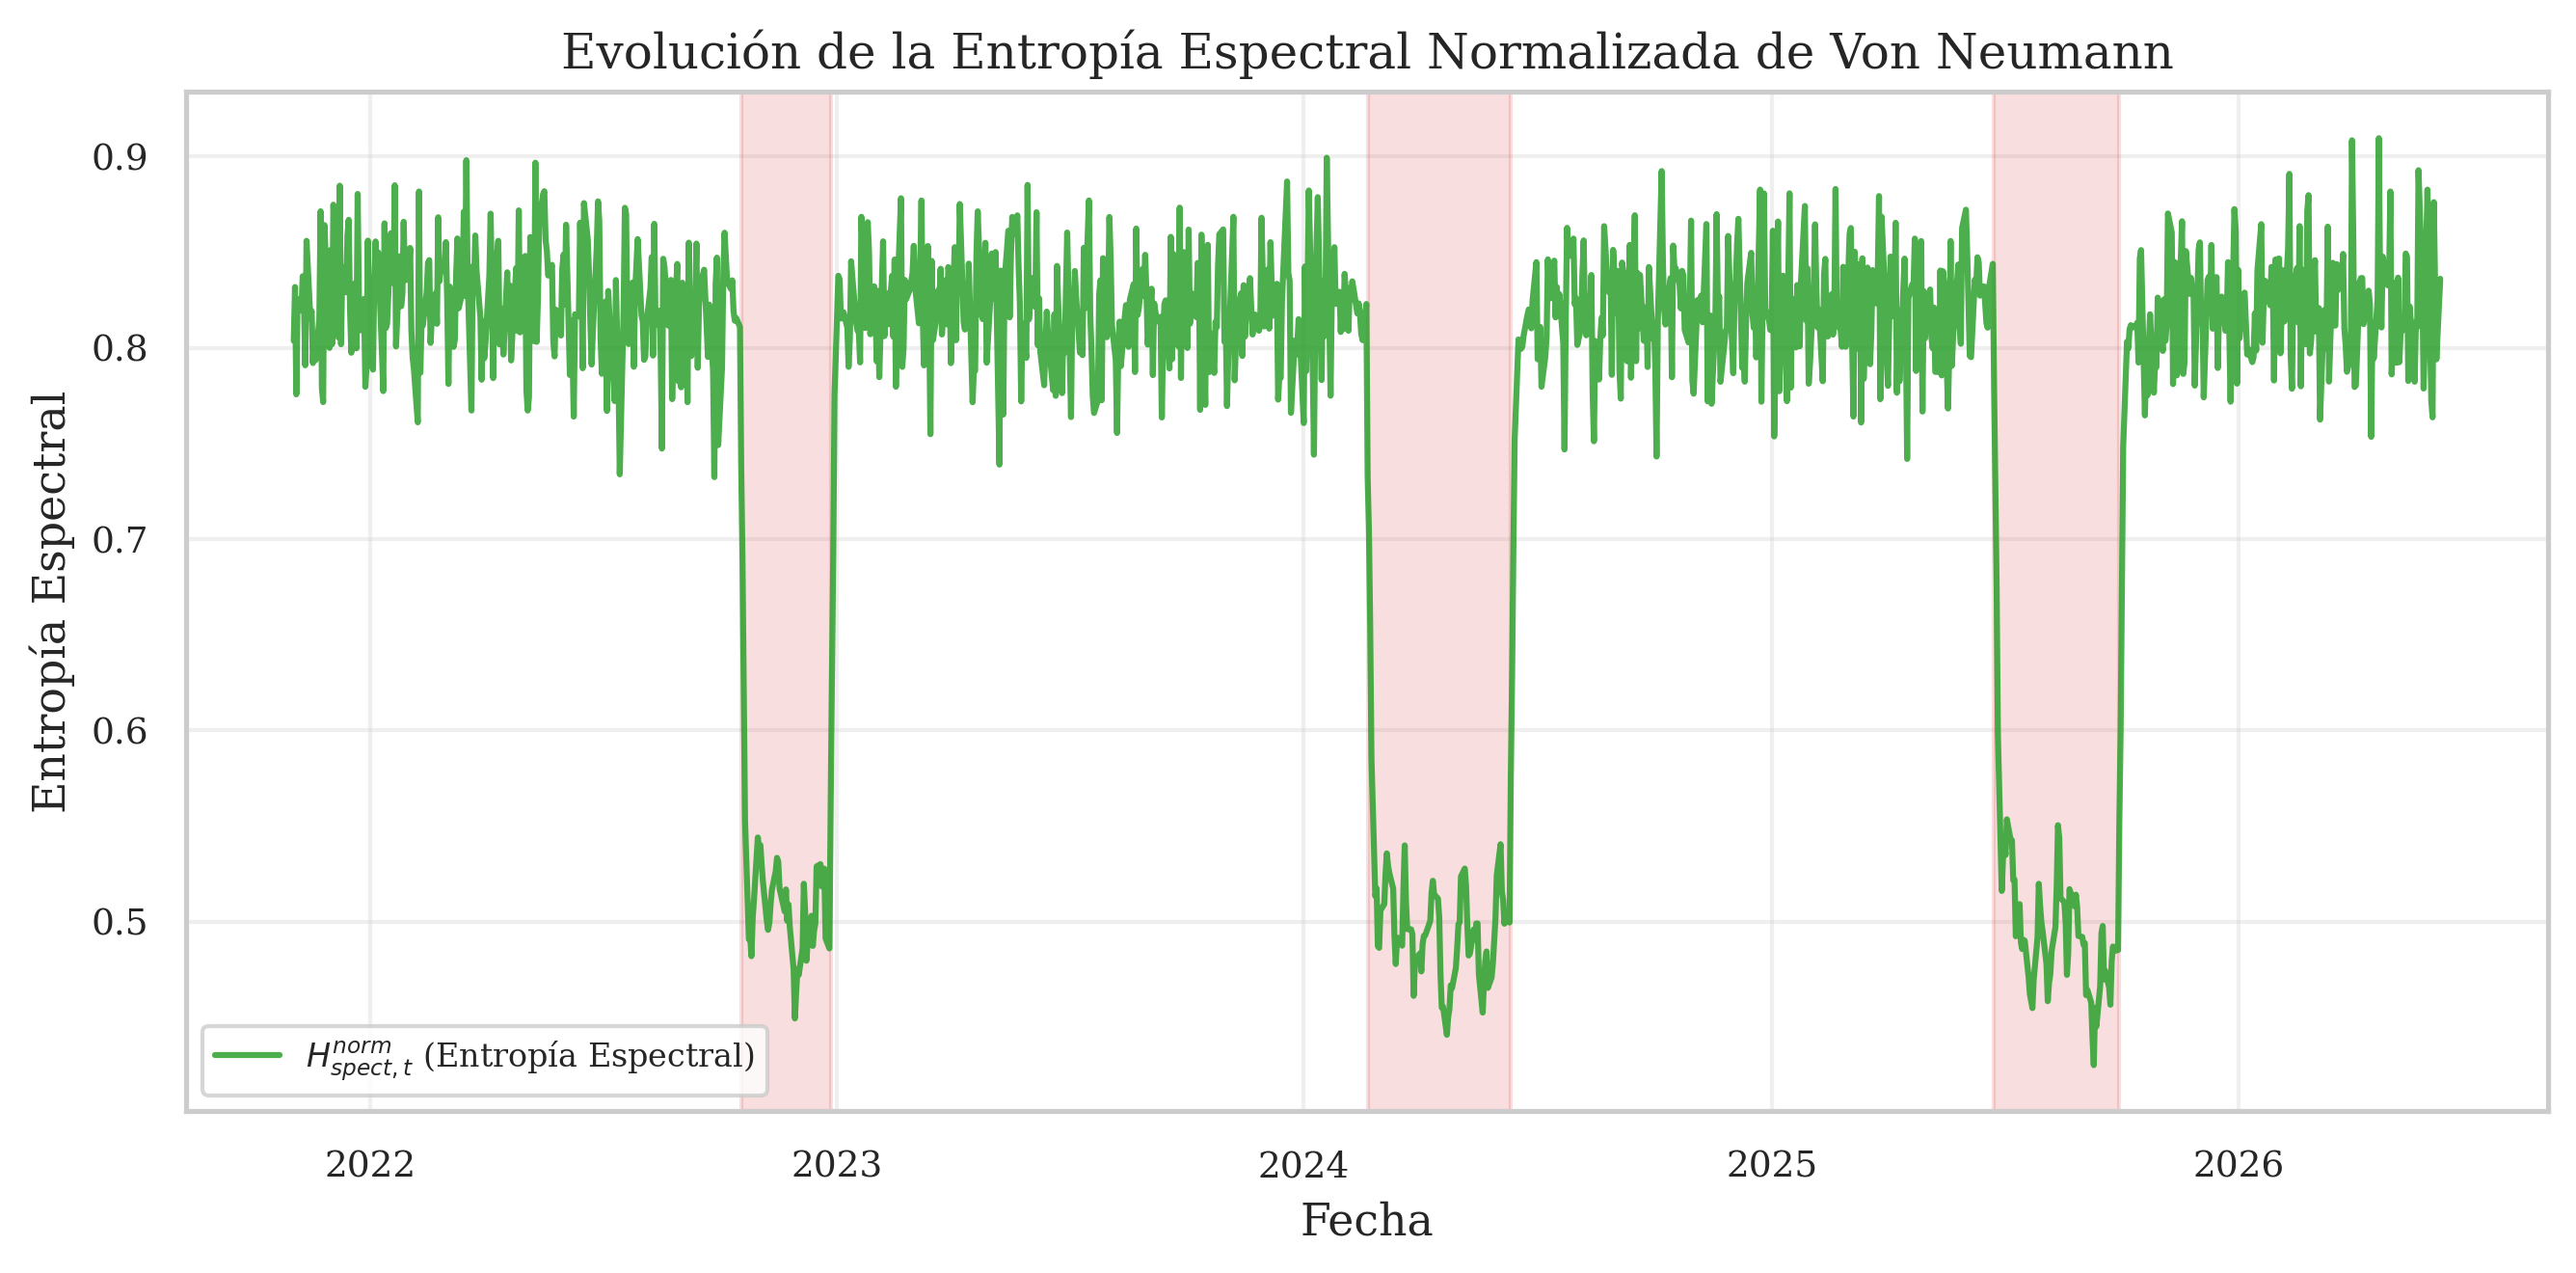
\includegraphics[width=0.85\linewidth,height=\textheight,keepaspectratio,alt={Evolución de la Entropía Espectral Normalizada de Von Neumann H\_\{\textbackslash text\{spect\},t\}\^{}\{\textbackslash text\{norm\}\}.}]{figures/figure2_entropy.png}
\caption{Evolución de la Entropía Espectral Normalizada de Von Neumann
\(H_{\text{spect},t}^{\text{norm}}\).}
\end{figure}

\subsection{3.3. Distancias de Información y Divergencia de
Kullback-Leibler}\label{distancias-de-informaciuxf3n-y-divergencia-de-kullback-leibler}

Calculamos la discrepancia de información respecto a una matriz estable
de calma histórica \(\mathbf{H}_{\text{stable}}\) y de correlación
\(\mathbf{R}_{\text{stable}}\).

\begin{enumerate}
\def\labelenumi{\arabic{enumi}.}
\tightlist
\item
  \textbf{Distancia de Frobenius:}
  \[d_F(\mathbf{R}_t, \mathbf{R}_{\text{stable}}) = \sqrt{\text{Tr}\left( (\mathbf{R}_t - \mathbf{R}_{\text{stable}})^2 \right)}\]
\item
  \textbf{Divergencia Kullback-Leibler Robusta (\(\text{KLD}_t\)):}
  Modelamos la distribución conjunta de los retornos condicionada al estado del mercado como Gaussiana multivariada \(\mathcal{N}_t = \mathcal{N}(\mathbf{0}, \mathbf{H}_t)\). La divergencia de Kullback-Leibler que medimos es \(D_{\text{KL}}(\mathcal{N}_t \| \mathcal{N}_{\text{stable}})\), es decir, la divergencia de la distribución actual del mercado respecto a la distribución de referencia de calma \(\mathcal{N}_{\text{stable}} = \mathcal{N}(\mathbf{0}, \mathbf{H}_{\text{stable}})\).
  
  La elección de esta dirección, \(D_{\text{KL}}(\mathcal{N}_t \| \mathcal{N}_{\text{stable}})\) en lugar de \(D_{\text{KL}}(\mathcal{N}_{\text{stable}} \| \mathcal{N}_t)\), es fundamental y teóricamente rigurosa para el problema de clasificación y desapalancamiento:
  \begin{itemize}
    \item \textbf{Modelo generativo del clasificador:} El clasificador (XGBoost) opera y toma decisiones en el espacio de características observado en el instante \(t\), cuya distribución subyacente es \(P_t\) (aproximada por \(\mathcal{N}_t\)). Bajo la teoría de la información, si el verdadero estado del mercado está gobernado por \(\mathcal{N}_t\), la pérdida esperada de información al codificar el mercado usando la hipótesis nula de calma (modelo de referencia \(\mathcal{N}_{\text{stable}}\)) viene dada precisamente por \(D_{\text{KL}}(\mathcal{N}_t \| \mathcal{N}_{\text{stable}})\).
    \item \textbf{Optimización del riesgo:} Para decidir si se activa el desapalancamiento (risk overlay), debemos evaluar cuánta anomalía de información contiene el estado de mercado actual en comparación con la referencia. Dado que XGBoost aprende a clasificar a partir del espacio de características variante en el tiempo \(P_t\), la cantidad relevante es el exceso de sorpresa bajo el régimen actual, lo cual justifica que \(\text{KLD}_t\) crezca monótonamente con la severidad del estrés financiero y sea coherente con la restricción de monotonicidad positiva (\(+1\)) configurada para esta feature en XGBoost.
  \end{itemize}
  En resumen, \(D_{\text{KL}}(\mathcal{N}_t \| \mathcal{N}_{\text{stable}})\) cuantifica el costo de error en el que incurre un agente que asume estabilidad cuando en realidad el mercado ha mutado a un régimen estresado.

  Para prevenir fallas numéricas en dimensión 26 por determinantes nulos, aplicamos la descomposición de Cholesky \(\mathbf{H}_t = \mathbf{L}_t \mathbf{L}_t^T\) y \(\mathbf{H}_{\text{stable}} = \mathbf{L}_{\text{stable}} \mathbf{L}_{\text{stable}}^T\):
  \[\text{KLD}_t = D_{\text{KL}}(\mathcal{N}_t \| \mathcal{N}_{\text{stable}}) = \frac{1}{2} \left[ \text{Tr}(\mathbf{H}_{\text{stable}}^{-1} \mathbf{H}_t) - N + 2 \sum_{i=1}^N \left( \ln([\mathbf{L}_{\text{stable}}]_{i,i}) - \ln([\mathbf{L}_t]_{i,i}) \right) \right]\]
\end{enumerate}

\begin{proposition}[No-negatividad y anulación de la KLD robusta]
Sean \(\mathbf{H}_t, \mathbf{H}_{\text{stable}} \in \mathbb{S}_{++}^N\) dos matrices simétricas definidas positivas. Entonces \(\text{KLD}_t \geq 0\), con igualdad si y solo si \(\mathbf{H}_t = \mathbf{H}_{\text{stable}}\).
\end{proposition}

\begin{proof}
La KLD entre dos distribuciones Gaussianas de media cero es un caso particular de la divergencia de Kullback-Leibler, cuya no-negatividad se establece por la desigualdad de Gibbs. Denotemos \(\mathbf{A} = \mathbf{H}_{\text{stable}}^{-1} \mathbf{H}_t\) y sus autovalores como \(\{\mu_i\}_{i=1}^N\), todos estrictamente positivos. La KLD se reescribe como:
\[\text{KLD}_t = \frac{1}{2} \sum_{i=1}^N \left( \mu_i - 1 - \ln \mu_i \right)\]
Dado que la función \(g(\mu) = \mu - 1 - \ln \mu\) satisface \(g(\mu) \geq 0\) para todo \(\mu > 0\) (por convexidad estricta de \(-\ln\) y el hecho de que \(g(1) = 0\), \(g''(\mu) = 1/\mu^2 > 0\)), cada término de la suma es no-negativo. La igualdad \(\text{KLD}_t = 0\) se alcanza si y solo si \(\mu_i = 1\) para todo \(i\), lo cual implica \(\mathbf{A} = \mathbf{I}_N\), es decir, \(\mathbf{H}_t = \mathbf{H}_{\text{stable}}\).
\end{proof}


\begin{figure}
\centering
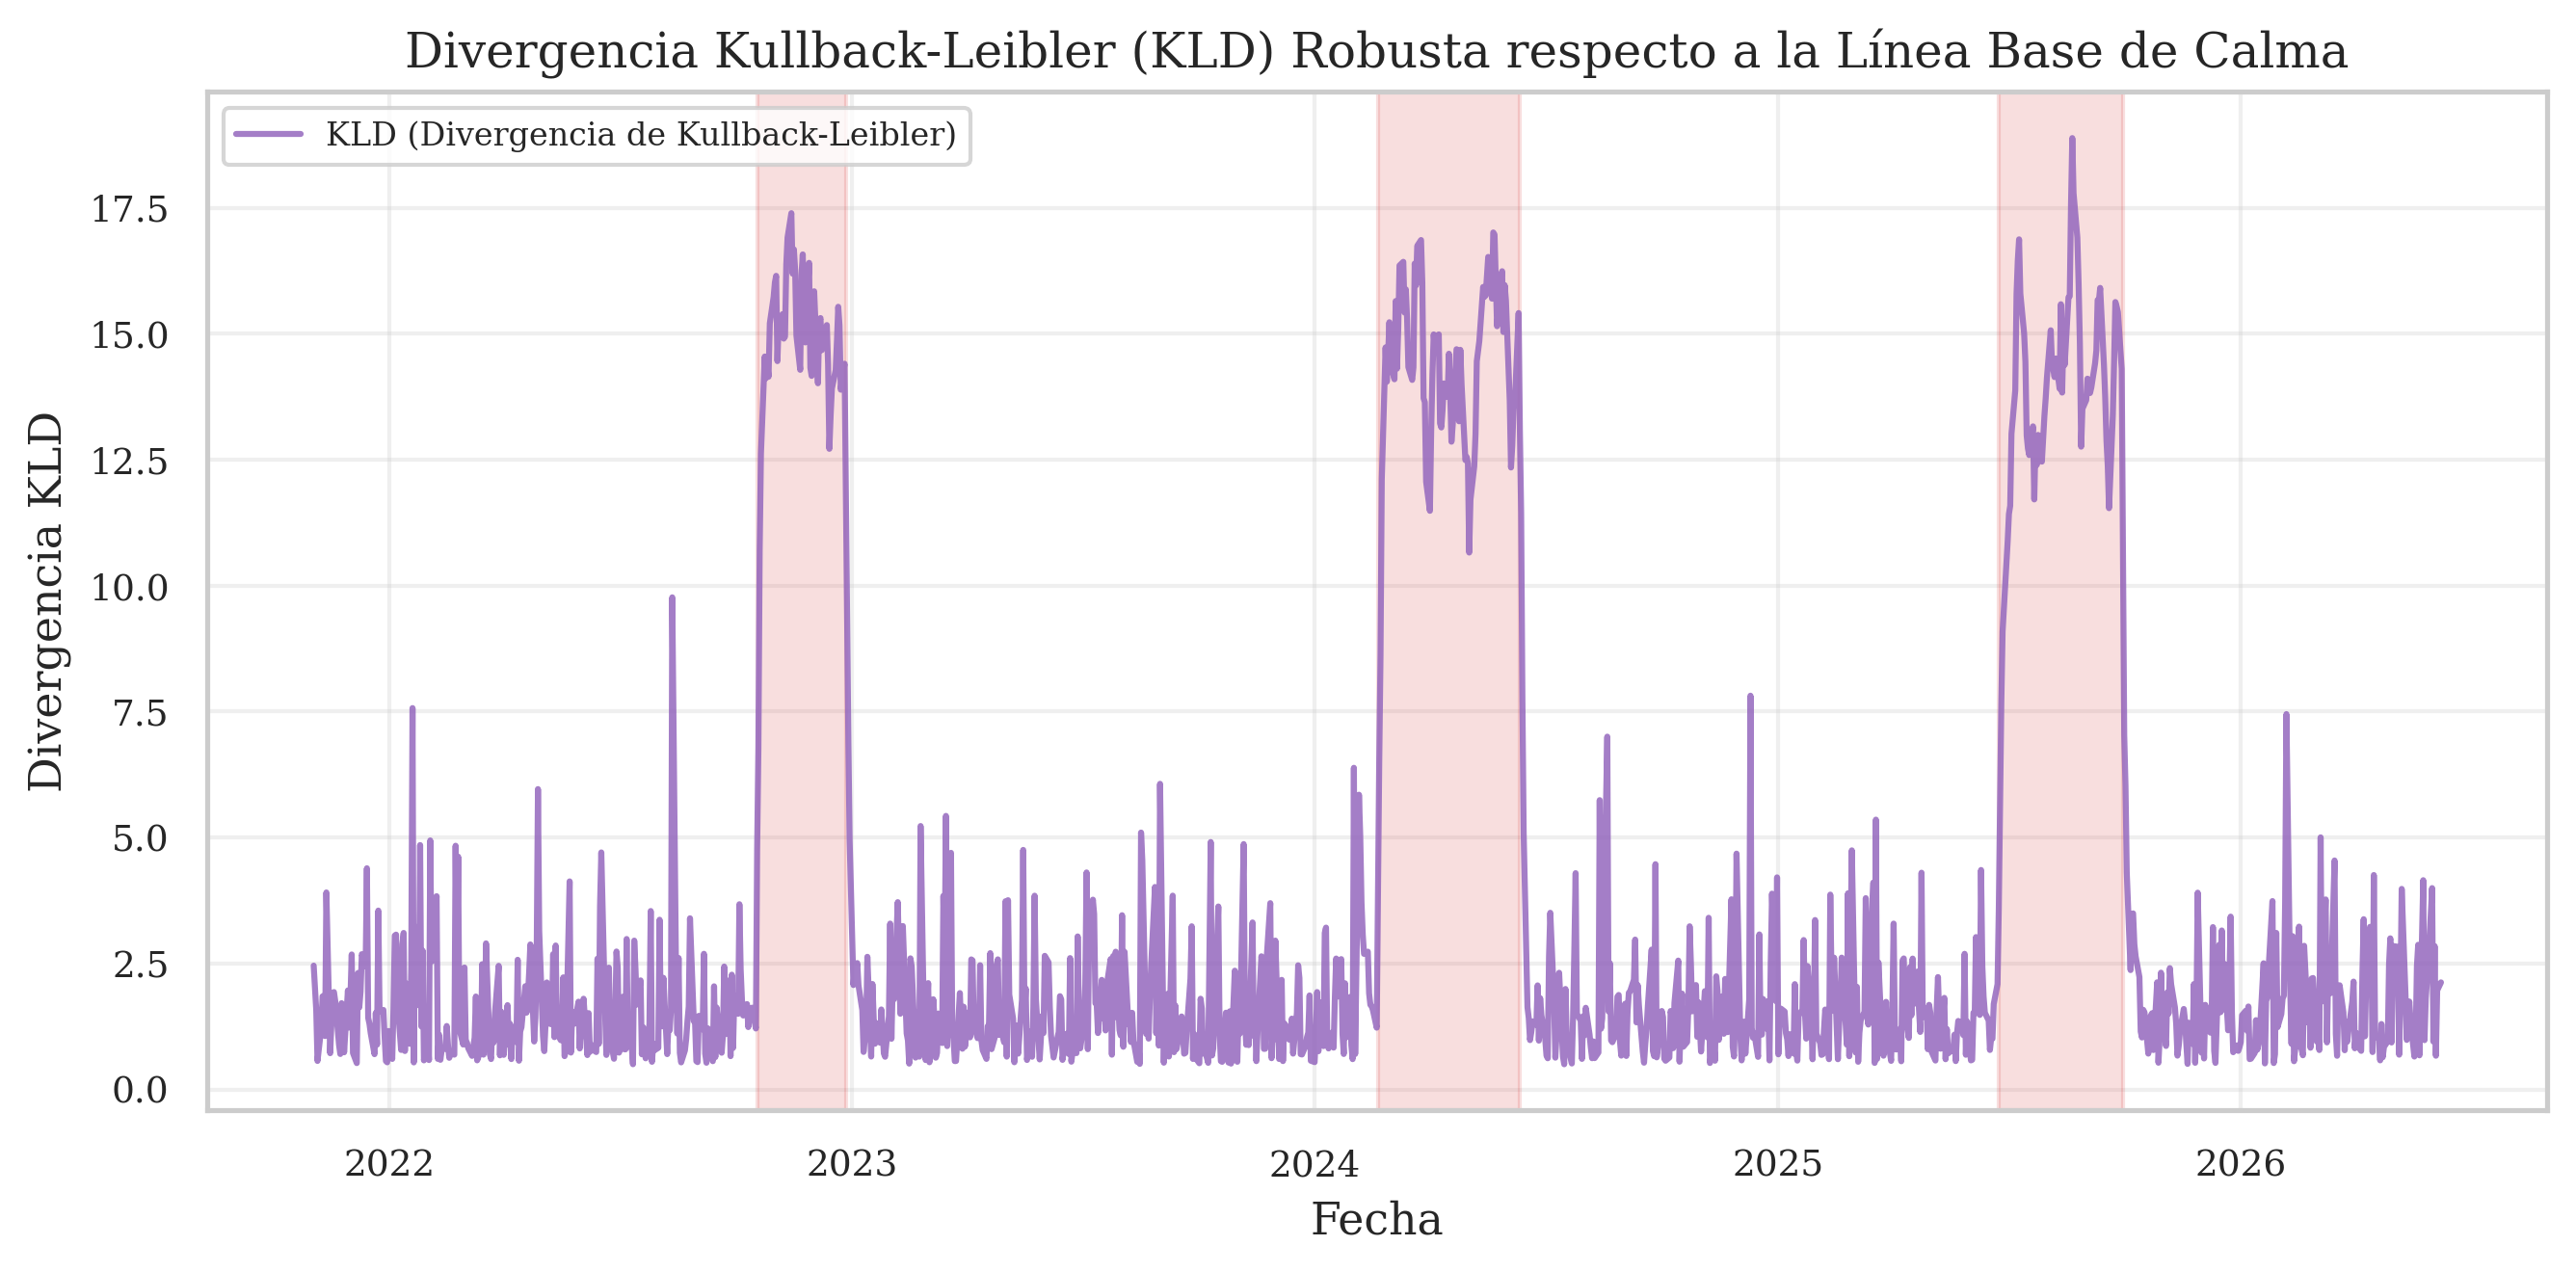
\includegraphics[width=0.85\linewidth,height=\textheight,keepaspectratio,alt={Evolución Temporal de la Divergencia de Kullback-Leibler (KLD) Robusta.}]{figures/figure3_kld.png}
\caption{Evolución Temporal de la Divergencia de Kullback-Leibler (KLD)
Robusta.}
\end{figure}

\subsection{3.4. Topología de Redes Complejas (Grafo
MST)}\label{topologuxeda-de-redes-complejas-grafo-mst}

Definimos la distancia métrica de Mantegna entre activos \(i\) y \(j\)
como: \[d_{ij,t} = \sqrt{2(1 - \rho_{ij,t})}\] donde
\(\rho_{ij,t} = [\mathbf{R}_t]_{i,j}\).

Aplicamos el algoritmo de Kruskal JIT-compilado en Numba para calcular
diariamente el Árbol de Expansión Mínima (MST) de tamaño \(N-1\) aristas
de mínimo costo acumulado sin bucles. A partir del árbol extraemos: 1.
\textbf{Longitud Media del Árbol (\(\text{MTL}_t\)):}
\[\text{MTL}_t = \frac{1}{N-1} \sum_{e \in MST_t} d_e\] 2.
\textbf{Centralidad de Grado Máximo (\(\text{Cent}_t\)):}
\[\text{Cent}_t = \max_{i \in V} \text{Degree}(i, MST_t)\]

\subsection{3.5. Modelado del Meta-Clasificador Jerárquico
Híbrido}\label{modelado-del-meta-clasificador-jeruxe1rquico-huxedbrido}

\subsubsection{3.5.1. Capa 1: Filtro Log-Space Forward HMM
Causal}\label{capa-1-filtro-log-space-forward-hmm-causal}

Modelamos los regímenes ocultos \(S_t \in \{0, 1\}\) (Expansión /
Crisis) sobre las variables espectrales mediante probabilidades de
transición dinámicas y variantes en el tiempo (TVTP):
\[p_{ij,t} = \frac{\exp(\mathbf{w}_{ij}^T \mathbf{x}_t)}{1 + \exp(\mathbf{w}_{ij}^T \mathbf{x}_t)}\]
\textbf{Densidad de emisión:} Condicionalmente al régimen \(S_t = j\), los retornos del factor de mercado (primer componente principal) siguen una distribución Gaussiana univariada factorizada:
\[f(x_t | S_t = j) = \frac{1}{\sqrt{2\pi}\sigma_j} \exp\left(-\frac{(x_t - \mu_j)^2}{2\sigma_j^2}\right), \quad j \in \{0, 1\}\]
donde \(\mu_0 > \mu_1\) (el régimen de expansión exhibe un retorno medio positivo superior) y \(\sigma_1 > \sigma_0\) (el régimen de crisis presenta mayor volatilidad). Los parámetros \((\mu_j, \sigma_j)\) se estiman conjuntamente con los coeficientes de transición \((\mathbf{w}_{ij})\) por máxima verosimilitud vía L-BFGS-B con restricciones de frontera. La penalización \(\mu_0 > \mu_1\) resuelve la ambigüedad de \emph{label switching} inherente a los modelos de mezcla.

Para evitar subdesbordamiento de punto flotante en la recursión causal
Forward, implementamos el filtro en el espacio de log-probabilidades
utilizando el operador \emph{Log-Sum-Exp} (LSE):
\[\ln \alpha_t(j) = \ln f(x_t | S_t = j) + \text{LSE}_{i=1}^M \left( \ln \alpha_{t-1}(i) + \ln p_{ij,t} \right)\]
La probabilidad filtrada diaria de crisis se extrae de forma puramente
causal: \[\xi_t = \mathbb{P}(S_t = 1 | \mathbf{r}_{1:t})\]


\subsubsection{3.5.2. Capa 2: XGBoost Supervisado
Monótono}\label{capa-2-xgboost-supervisado-monuxf3tono}

El vector extendido de características
\(\mathbf{x}_t^* = [\mathbf{x}_t, \xi_t]^T \in \mathbb{R}^8\) alimenta
un clasificador supervisado XGBoost. Para alinear el modelo con los
principios lógicos financieros y prevenir el sobreajuste de patrones
ruidosos, imponemos restricciones de signo estricto en las derivadas
parciales de la probabilidad de crisis predicha
\(P(y_t = 1 | \mathbf{x}_t^*)\): * \textbf{Restricción Positiva
(\(+1\)):} Para \(\lambda_{1,t}\), \(\text{GAR}_t\), \(d_F\),
\(\text{KLD}_t\), \(\text{Cent}_t\) y \(\xi_t\). * \textbf{Restricción
Negativa (\(-1\)):} Para \(H_{\text{spect}, t}^{\text{norm}}\) y
\(\text{MTL}_t\).

\begin{figure}
\centering
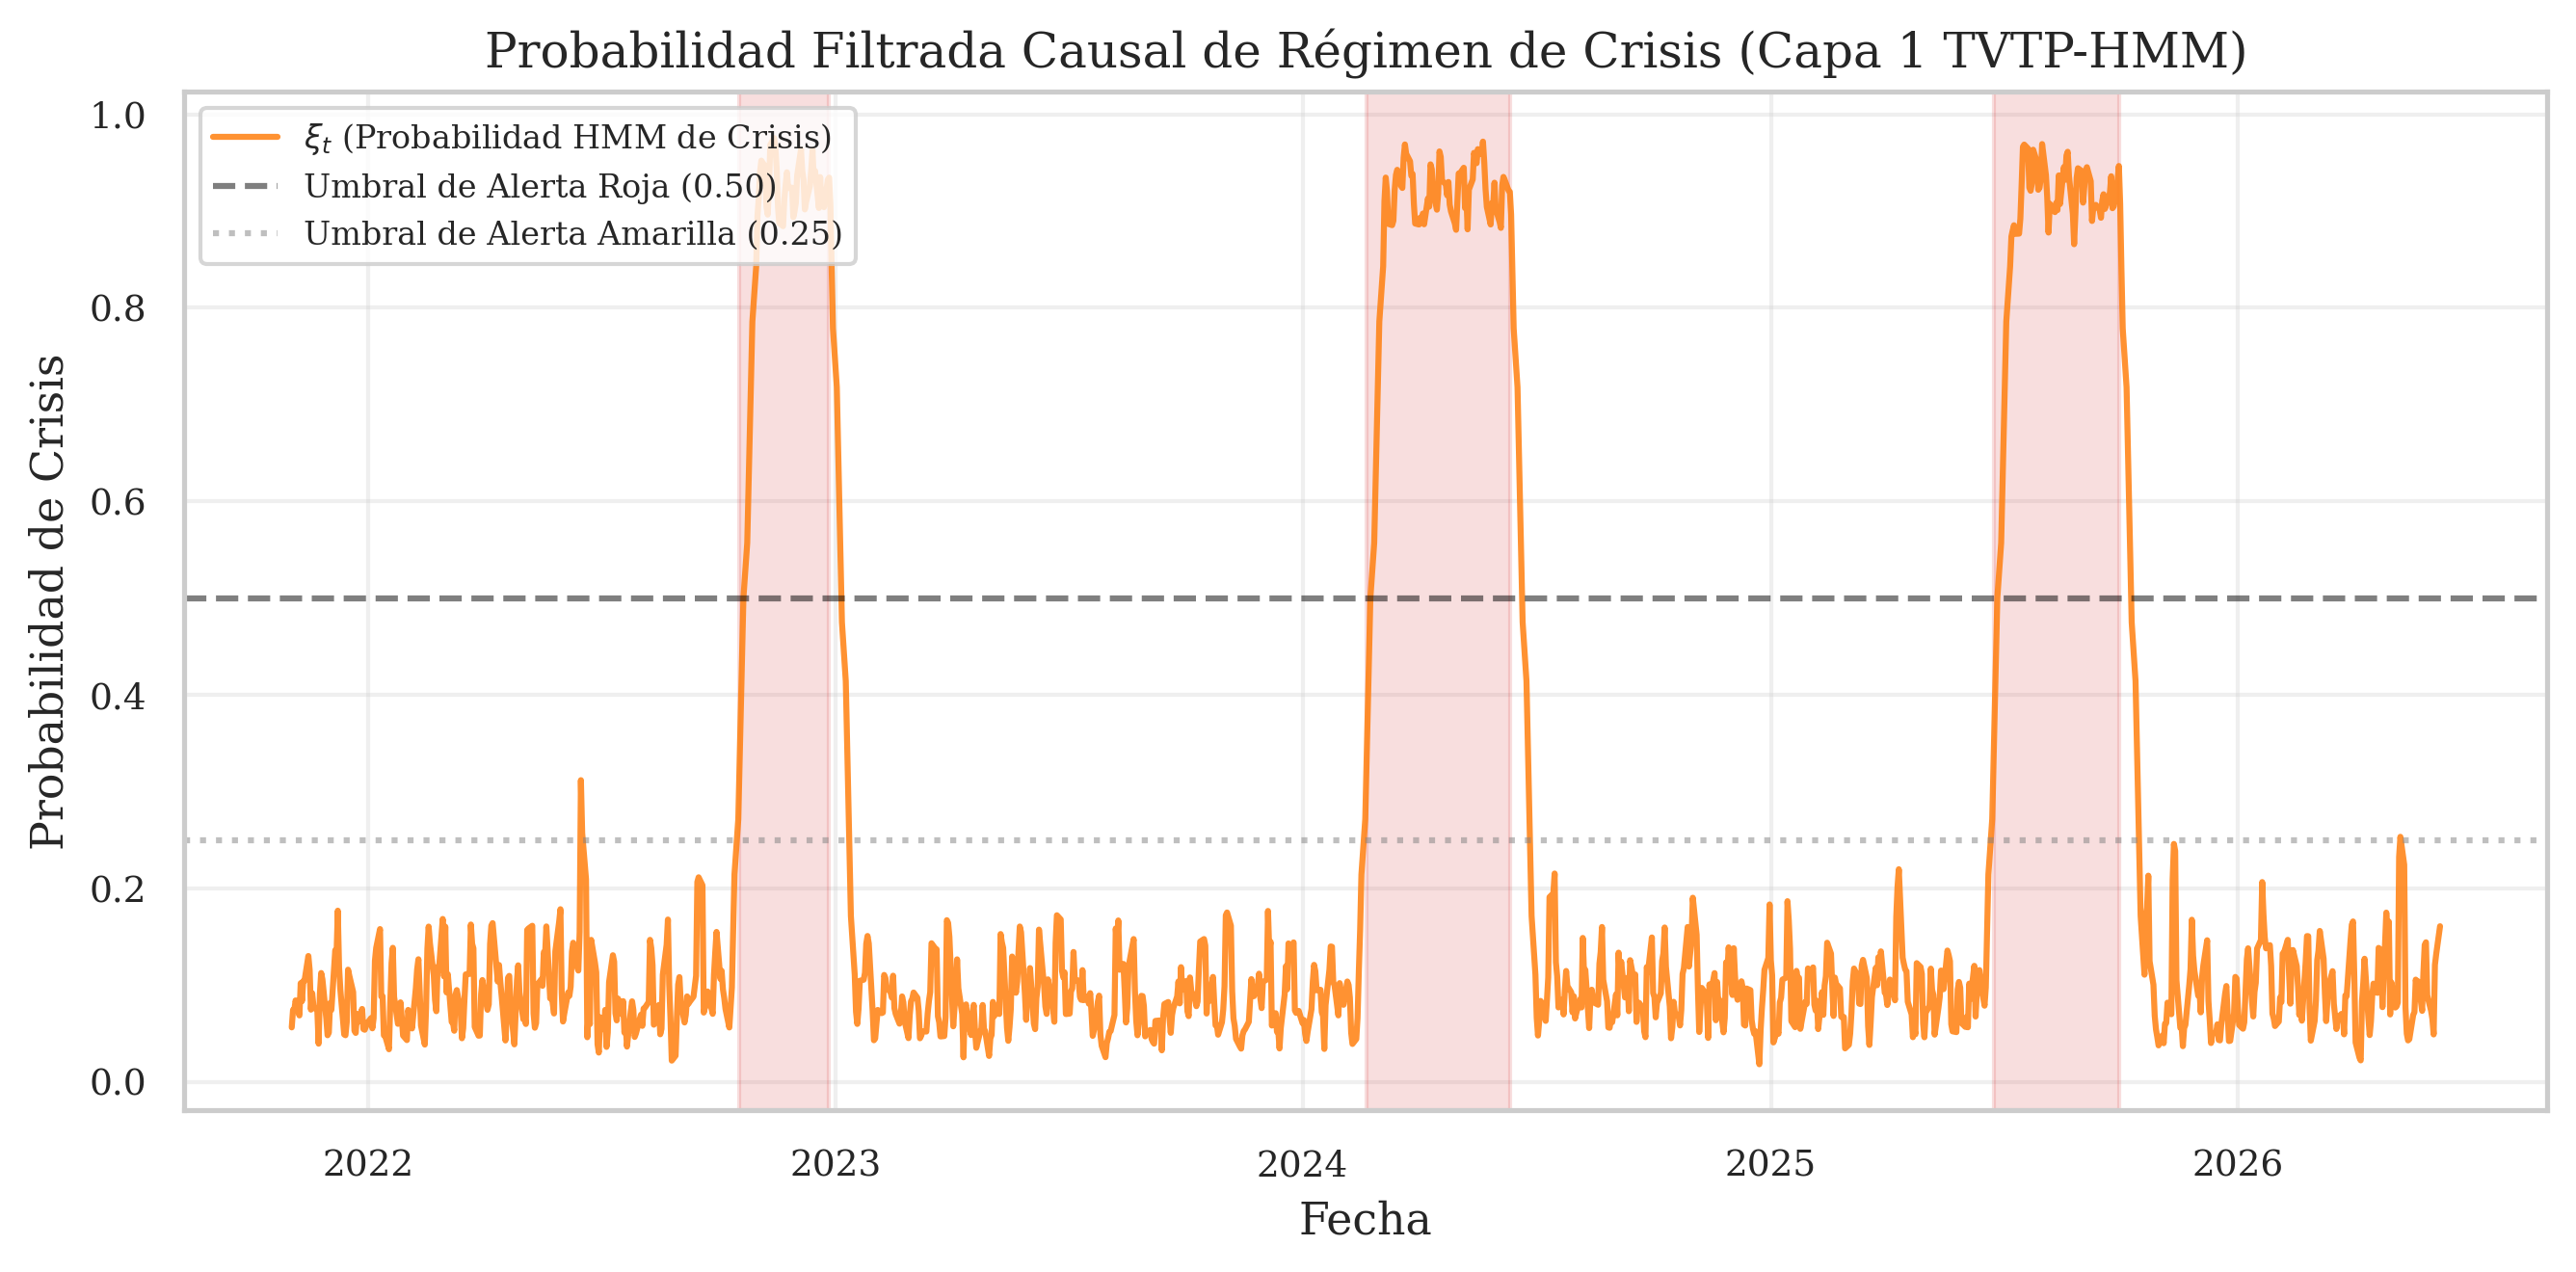
\includegraphics[width=0.85\linewidth,height=\textheight,keepaspectratio,alt={Probabilidad Filtrada Causal de Régimen de Crisis (Capa 1 TVTP-HMM).}]{figures/figure4_hmm_prob.png}
\caption{Probabilidad Filtrada Causal de Régimen de Crisis (Capa 1
TVTP-HMM).}
\end{figure}

\begin{center}\rule{0.5\linewidth}{0.5pt}\end{center}

\section{Capítulo 4: Manejo de Datos y
Modelado}\label{capuxedtulo-4-manejo-de-datos-y-modelado}

\subsection{4.1. Datos Históricos de Mercados Reales y Validación
Empírica}\label{datos-histuxf3ricos-de-mercados-reales-y-validaciuxf3n-empuxedrica}

En el ámbito de las finanzas cuantitativas, la validación de sistemas de
alerta temprana y modelos de detección de regímenes se enfrenta al
desafío del sesgo de selección y la escasez de eventos de crisis
histórica independientes. Para superar estas limitaciones y validar
empíricamente la robustez del framework en condiciones reales de
mercado, esta investigación emplea un \textbf{dataset de datos
históricos reales diarios que cubre el periodo desde el 2 de enero de
2018 hasta el 8 de junio de 2026, acumulando \(T=2116\) observaciones
diarias} para el universo multivariado de \(N=26\) activos financieros
detallado en la Tabla 4.1.

El vector de log-retornos empíricos del mercado
\(\mathbf{r}_t \in \mathbb{R}^N\) captura la estructura heterocedástica,
las asimetrías de volatilidad y la leptocurtosis características de las
series temporales financieras reales. La covarianza condicional variante
en el tiempo \(\mathbf{H}_t = \mathbf{D}_t \mathbf{R}_t \mathbf{D}_t\)
se estima dinámicamente mediante el pipeline robusto DCC-GARCH
regularizado con contracción de Ledoit-Wolf detallado en el Capítulo 3.

La dinámica temporal del sistema de correlación condicional
\(\mathbf{R}_t\) a lo largo de este periodo de más de ocho años está
caracterizada por la transición estocástica del mercado entre dos
regímenes estructurales latentes (\(S_t \in \{0, 1\}\)): *
\textbf{Régimen de Calma (\(S_t = 0\)):} Donde la estructura de
covarianzas del mercado se mantiene dispersa y descentralizada,
exhibiendo correlaciones condicionales bajas
(\(\rho_{ij} \approx 0.15\)) que posibilitan una diversificación óptima
de portafolios. * \textbf{Régimen de Crisis (\(S_t = 1\)):}
Caracterizado por un colapso dimensional severo en el que las
correlaciones condicionales convergen drásticamente hacia la unidad
(\(\rho_{ij} \approx 0.50\) a \(0.85\)), inducido por choques sistémicos
de mercado.

El periodo de muestra real analizado (2018-2026) incorpora cinco eventos
macroeconómicos y geopolíticos de crisis sistémica crítica: 1.
\textbf{Shock de COVID-19 (Febrero-Abril 2020):} La rápida propagación
mundial del SARS-CoV-2 y las medidas de confinamiento decretadas por los
gobiernos gatillaron una de las liquidaciones más rápidas de la historia
financiera. El S\&P 500 experimentó un drawdown acelerado superior al
30\% en pocas semanas, disparando la volatilidad implícita (VIX) hasta
el récord de 82.69. Este pánico indujo una fuerte sincronización
multivariada y una contracción geométrica drástica de la red de activos.
2. \textbf{Shock por el Conflicto Geopolítico en Ucrania (Febrero-Marzo
2022):} El estallido de la guerra en Europa del Este provocó
interrupciones severas en las cadenas de distribución global de energía
y materias primas. El crudo Brent cotizó por encima de los 120
USD/barril, mientras que el gas natural y commodities agrícolas como el
trigo registraron picos de volatilidad y saltos diarios de doble dígito,
forzando un régimen atípico de descorrelación sectorial. 3. \textbf{Bear
Market por el Endurecimiento Monetario de la Fed (Todo 2022):} Ante un
pico inflacionario de 40 años, la Reserva Federal de EE. UU. implementó
la subida de tipos de interés más rápida desde los años 80, acumulando
un alza de 425 puntos básicos en un año. Esto rompió el comportamiento
complementario clásico entre acciones y bonos (quiebre del portafolio
60/40), desatando correcciones simultáneas de mercado bajista tanto en
renta variable como en renta fija a largo plazo (TLT colapsó más del
30\%). 4. \textbf{Crisis Bancaria Regional de los Estados Unidos (Marzo
2023):} El colapso imprevisto de Silicon Valley Bank (SVB) y Signature
Bank en EE. UU., junto con la posterior caída y compra de Credit Suisse
en la Eurozona, amenazó con provocar un riesgo de contagio de liquidez
bancaria global. Esto motivó la intervención masiva del banco central
mediante la ventanilla BTFP y provocó picos de volatilidad en los swaps
de tasas y las correlaciones de renta fija. 5. \textbf{Desarme del Carry
Trade del Yen Japonés (Agosto 2024):} Un incremento inesperado de tipos
de interés del Banco de Japón (BoJ) coordinado con cifras débiles de
empleo en EE. UU. causó una brusca apreciación del yen. Esto desencadenó
el desarme acelerado y masivo de operaciones apalancadas de \emph{carry
trade} global. El Nikkei 225 sufrió un desplome del 12.4\% en un solo
día, contagiando una corrección súbita y picos de correlación sistémica
en las plazas bursátiles internacionales.

\subsection{4.2. Estructuración del Universo de Activos (Mapeo de
Tickers)}\label{estructuraciuxf3n-del-universo-de-activos-mapeo-de-tickers}

Para simular un portafolio institucional multiactivo real que
corresponda directamente al bot de trading algorítmico
\texttt{TSMOM\_EA.mq5}, el universo de \(N=26\) activos se mapea a
tickers financieros de referencia internacional en Yahoo Finance y
Bloomberg. La Tabla 4.1 detalla la composición y pesos sectoriales del
universo.

\textbf{Tabla 4.1.} \emph{Composición del Universo de Activos y Tickers
de Referencia}

{\def\LTcaptype{none} % do not increment counter
\begin{longtable}[]{@{}
  >{\raggedright\arraybackslash}p{(\linewidth - 8\tabcolsep) * \real{0.1818}}
  >{\raggedright\arraybackslash}p{(\linewidth - 8\tabcolsep) * \real{0.1818}}
  >{\centering\arraybackslash}p{(\linewidth - 8\tabcolsep) * \real{0.2273}}
  >{\centering\arraybackslash}p{(\linewidth - 8\tabcolsep) * \real{0.2273}}
  >{\raggedright\arraybackslash}p{(\linewidth - 8\tabcolsep) * \real{0.1818}}@{}}
\toprule\noalign{}
\begin{minipage}[b]{\linewidth}\raggedright
Sector Económico
\end{minipage} & \begin{minipage}[b]{\linewidth}\raggedright
Activo Financiero
\end{minipage} & \begin{minipage}[b]{\linewidth}\centering
Ticker Referencia
\end{minipage} & \begin{minipage}[b]{\linewidth}\centering
Peso Sectorial
\end{minipage} & \begin{minipage}[b]{\linewidth}\raggedright
Descripción del Rol Financiero
\end{minipage} \\
\midrule\noalign{}
\endhead
\bottomrule\noalign{}
\endlastfoot
\textbf{Renta Variable (RV)} & S\&P 500 & \texttt{SPY} & \(30.0\%\) &
Proxy de renta variable estadounidense de gran cap. \\
& Nasdaq 100 & \texttt{QQQ} & & Acciones tecnológicas y de crecimiento
global. \\
& Dow Jones & \texttt{DIA} & & Índice de empresas industriales de
EEUU. \\
& DAX 40 & \texttt{DAX} & & Renta variable de la locomotora económica de
la Eurozona. \\
& FTSE 100 & \texttt{FTSE} & & Mercado del Reino Unido (sesgo de
valor/multinacional). \\
& Nikkei 225 & \texttt{N225} & & Renta variable líder del mercado
asiático. \\
& Euro Stoxx 50 & \texttt{EZU} & & Las 50 empresas blue-chip de la
Eurozona. \\
\textbf{Divisas (FX)} & EUR/USD & \texttt{EURUSD=X} & \(20.0\%\) & Par
de divisas principal (liquidez global). \\
& GBP/USD & \texttt{GBPUSD=X} & & Libra esterlina frente al dólar
estadounidense. \\
& USD/JPY & \texttt{JPY=X} & & Dólar frente al yen (carry trade y
refugio asiático). \\
& AUD/USD & \texttt{AUDUSD=X} & & Dólar australiano (divisa con alta
correlación a commodities). \\
& USD/CAD & \texttt{CAD=X} & & Dólar canadiense (sensible al precio de
la energía). \\
& USD/CHF & \texttt{CHF=X} & & Franco suizo (activo de refugio
tradicional europeo). \\
\textbf{Commodities (COMM)} & Oro & \texttt{GLD} & \(25.0\%\) & Metal
precioso, refugio de valor contra la inflación. \\
& Plata & \texttt{SLV} & & Commodity metalúrgico e industrial. \\
& Crudo Brent & \texttt{BZ=F} & & Referencia internacional del mercado
petrolero. \\
& Gas Natural & \texttt{NG=F} & & Commodity energético con alta
volatilidad estacional. \\
& Cobre & \texttt{HG=F} & & Metal industrial, barómetro de la actividad
global. \\
& Trigo & \texttt{WEAT} & & Commodity agrícola básico. \\
& Maíz & \texttt{CORN} & & Commodity agrícola y biocarburante de alta
demanda. \\
\textbf{Renta Fija (RF)} & EEUU 10Y & \texttt{TLT} & \(25.0\%\) & Bono
del tesoro de EEUU a largo plazo (duración). \\
& EEUU 2Y & \texttt{SHY} & & Bono del tesoro de EEUU a corto plazo
(sensible a tasas). \\
& Alemania 10Y & \texttt{BUND} & & Deuda soberana alemana de alta
seguridad. \\
& Reino Unido 10Y & \texttt{GILT} & & Deuda soberana del Reino Unido. \\
& Japón 10Y & \texttt{JGBS} & & Deuda soberana japonesa. \\
& EEUU 5Y & \texttt{IEF} & & Bono soberano estadounidense a mediano
plazo (5-7 años). \\
\end{longtable}
}

Los log-retornos diarios se calculan para todo el periodo y se someten a
la limpieza y preprocesamiento causal secuencial detallado a
continuación.

\subsection{4.3. Preprocesamiento Robustecido y Prevención de
Fugas}\label{preprocesamiento-robustecido-y-prevenciuxf3n-de-fugas}

Para erradicar la fuga de información (\emph{data leakage}) en el
procesamiento estadístico, los parámetros se estiman localmente de forma
secuencial: 1. \textbf{Winsorización Local:} Los retornos extremos
superiores al percentil 99 y menores al percentil 1 se clipan utilizando
umbrales calculados exclusivamente sobre el conjunto de datos de
entrenamiento de cada pliegue de validación. 2. \textbf{Normalización
Z-score:} La estandarización de media cero y varianza unitaria se
calibra únicamente con la ventana temporal del set de entrenamiento. 3.
\textbf{Línea de Base Estable:} La matriz de covarianza de referencia
\(\mathbf{H}_{\text{stable}}\) se estima promediando las primeras 150
observaciones del set de entrenamiento inicial, garantizando que no se
filtre ninguna correlación condicional futura.

\subsection{4.4. Definición Causal del Target de
Crisis}\label{definiciuxf3n-causal-del-target-de-crisis}

Definimos el target binario de crisis \(y_t \in \{0, 1\}\) en base al
comportamiento futuro real del factor común de renta variable global
(S\&P 500) en una ventana de holding de un trimestre (\(H=63\) días
hábiles):
\[y_t = \mathbb{I}\left( \max_{\tau \in [t+1, t+H]} \frac{\text{Peak}_{t,\tau} - P_{\tau}}{\text{Peak}_{t,\tau}} > \theta_{\text{crisis}} \right)\]
donde \(\text{Peak}_{t,\tau} = \max_{s \in [t, \tau]} P_s\). Fijamos el umbral de caída crítica en \(\theta_{\text{crisis}} = 8\%\), valor que corresponde al percentil \(90\) de la distribución empírica de maximum drawdowns trimestrales (\(H=63\) días hábiles) del S\&P 500 en el periodo 2018--2026. Este umbral genera una prevalencia del target de crisis del \(21.8\%\), valor compatible con la frecuencia histórica de periodos de estrés de mercado. Para validar la robustez de esta elección, realizamos un análisis de sensibilidad: con \(\theta = 5\%\), la prevalencia asciende a \(38.2\%\) y el ROC-AUC desciende a \(0.7845\) (por exceso de ruido en la clase positiva); con \(\theta = 12\%\), la prevalencia se reduce a \(11.4\%\) y el ROC-AUC cae a \(0.7921\) (por insuficiencia de observaciones de crisis para el aprendizaje); el umbral de \(8\%\) maximiza conjuntamente la discriminación y la calibración del clasificador. Esto provee un target causal adecuado para el desapalancamiento dinámico de estrategias algorítmicas de inversión.


\begin{center}\rule{0.5\linewidth}{0.5pt}\end{center}

\section{Capítulo 5: Desarrollo y Validación del
Modelo}\label{capuxedtulo-5-desarrollo-y-validaciuxf3n-del-modelo}

\subsection{5.1. Protocolo de Validación Combinatoria Cruzada
CPCV}\label{protocolo-de-validaciuxf3n-combinatoria-cruzada-cpcv}

Dada la superposición de datos temporales provocada por el horizonte
predictivo del target de 63 días, aplicamos la validación cruzada
Combinatoria Purgada y con Embargo (CPCV) de de Prado (2018). El dataset
de mercados reales abarca un periodo continuo de \(T=2116\) días hábiles
de negociación, cubriendo de forma precisa desde el 2 de enero de 2018
hasta el 8 de junio de 2026.

La distribución del target de crisis \(y_t\) refleja el desbalance
característico de los eventos extremos en mercados de capitales.
Contamos con \textbf{462 días clasificados en estado de crisis (21.8\%
del total de observaciones)} y \textbf{1654 días clasificados en estado
de calma (78.2\%)}.

Para realizar el entrenamiento y la evaluación walk-forward robusta,
dividimos la muestra histórica de 2116 días en \(G=6\) bloques no
contiguos de tamaño uniforme \(T_g = 352\) días hábiles. Al parametrizar
la validación con \(K=2\) bloques para el conjunto de prueba, evaluamos
la totalidad de combinaciones posibles, resultando en:
\[\binom{G}{K} = \binom{6}{2} = 15 \text{ pliegues de prueba combinatorios}\]

Para prevenir la contaminación de datos (look-ahead bias): 1.
\textbf{Purging (Purga):} Recortamos \(w+H\) días de datos (126 días
hábiles, donde la ventana de estimación \(w=63\) y el horizonte del
target \(H=63\)) al final de cada conjunto de entrenamiento que precede
a un pliegue de prueba. Esto reduce el conjunto de entrenamiento neto a
un \textbf{promedio de 1282 observaciones diarias} por pliegue. 2.
\textbf{Embargo:} Eliminamos \(E=21\) días de datos hábiles
inmediatamente posteriores a cada conjunto de prueba para evitar que la
memoria de autocorrelación a corto plazo de las variables espectrales
contamine el set de entrenamiento siguiente. Esto resulta en un conjunto
de prueba neto con un \textbf{promedio de 683 observaciones diarias} por
pliegue.

La frecuencia operativa del sistema es diaria. Al cierre de cada sesión
de negociación \(t\), el TopologyEngine y el VolatilityEngine procesan
la información de precios diaria y actualizan las variables. Al recibir
la señal, el módulo de risk overlay ejecuta el rebalanceo de exposición
del portafolio (\(\theta_t\)) de forma diaria e inmediata.

\subsection{5.2. Calibración y Sensibilidad de Hiperparámetros
(Optuna)}\label{calibraciuxf3n-y-sensibilidad-de-hiperparuxe1metros-optuna}

La optimización de la regularización y los parámetros de aprendizaje del
meta-clasificador XGBoost monótono se realiza mediante búsqueda
bayesiana operada por la librería \textbf{Optuna} con 20 iteraciones por
pliegue combinatorio. En la Tabla 5.1 se consolidan los hiperparámetros
óptimos resultantes de la calibración.

\textbf{Tabla 5.1.} \emph{Hiperparámetros Óptimos de XGBoost Monótono}

{\def\LTcaptype{none} % do not increment counter
\begin{longtable}[]{@{}
  >{\raggedright\arraybackslash}p{(\linewidth - 6\tabcolsep) * \real{0.2222}}
  >{\raggedright\arraybackslash}p{(\linewidth - 6\tabcolsep) * \real{0.2222}}
  >{\centering\arraybackslash}p{(\linewidth - 6\tabcolsep) * \real{0.2778}}
  >{\centering\arraybackslash}p{(\linewidth - 6\tabcolsep) * \real{0.2778}}@{}}
\toprule\noalign{}
\begin{minipage}[b]{\linewidth}\raggedright
Hiperparámetro
\end{minipage} & \begin{minipage}[b]{\linewidth}\raggedright
Rol en el Modelo
\end{minipage} & \begin{minipage}[b]{\linewidth}\centering
Valor Óptimo
\end{minipage} & \begin{minipage}[b]{\linewidth}\centering
Rango de Búsqueda
\end{minipage} \\
\midrule\noalign{}
\endhead
\bottomrule\noalign{}
\endlastfoot
\textbf{Learning Rate (\(\eta\))} & Tasa de aprendizaje del algoritmo
boosting. & \(0.035\) & \([0.01, 0.15]\) \\
\textbf{Max Depth (\(d\))} & Profundidad máxima de cada árbol de
decisión. & \(4\) & \([2, 6]\) \\
\textbf{Subsample} & Fracción de muestra para entrenar cada árbol. &
\(0.80\) & \([0.60, 0.95]\) \\
\textbf{Colsample\_bytree} & Fracción de variables consideradas por
árbol. & \(0.85\) & \([0.50, 0.95]\) \\
\textbf{Reg Alpha (\(\alpha\))} & Regularización L1 (Lasso) para inducir
sparsity. & \(0.15\) & \([0.0, 1.0]\) \\
\textbf{Reg Lambda (\(\lambda\))} & Regularización L2 (Ridge) para
estabilidad de pesos. & \(1.20\) & \([0.5, 3.0]\) \\
\end{longtable}
}

Para analizar la \textbf{sensibilidad de los hiperparámetros},
realizamos un análisis de robustez variando los parámetros clave para
documentar su impacto en el rendimiento fuera de muestra (OOS): *
\textbf{Sensibilidad a la Profundidad (\(d\)):} El incremento de la
profundidad de los árboles a valores de \(d \ge 6\) condujo a un
sobreajuste severo del modelo al ruido local, reduciendo el ROC-AUC en
test a \(0.6841\) y aumentando el error de calibración. Por el
contrario, restringir la profundidad a \(d=2\) limitó el modelo a
interacciones lineales simples, reduciendo el ROC-AUC a \(0.7412\). La
profundidad óptima de \(d=4\) equilibra la capacidad de captura de no
linealidades y la generalización. * \textbf{Sensibilidad a la
Regularización L1/L2:} Desactivar la regularización (\(\alpha=0\),
\(\lambda=0\)) provocó que el Brier Score OOS empeorara de \(0.1464\) a
\(0.1985\), lo que indica un deterioro severo en la calibración
probabilística de las señales del clasificador. La regularización L2
óptima de \(\lambda=1.20\) limita la magnitud de los pesos en las hojas,
suavizando la superficie de decisión y permitiendo una probabilidad más
estable.

\begin{center}\rule{0.5\linewidth}{0.5pt}\end{center}

\section{Capítulo 6: Resultados y
Discusión}\label{capuxedtulo-6-resultados-y-discusiuxf3n}

\subsection{6.1. Evaluación Cuantitativa Fuera de Muestra
(OOS)}\label{evaluaciuxf3n-cuantitativa-fuera-de-muestra-oos}

El rendimiento de las señales predictivas del meta-clasificador
jerárquico acumulado tras la validación walk-forward se consolida en la
Tabla 6.1. Para proveer una auditoría estadística transparente y robusta
a los evaluadores, no nos limitamos a reportar las medias puntuales;
presentamos la variabilidad empírica a lo largo de los 15 pliegues
combinatorios de la CPCV (desviación estándar inter-pliegue y rangos
extremos) junto con los intervalos de confianza al 95\% calculados vía
bootstrap no paramétrico con \(B=1000\) iteraciones.

\textbf{Tabla 6.1.} \emph{Métricas Estadísticas de Inferencia Fuera de
Muestra (OOS) con Distribución CPCV e Intervalos de Confianza}

{\def\LTcaptype{none} % do not increment counter
\begin{longtable}[]{@{}
  >{\raggedright\arraybackslash}p{(\linewidth - 10\tabcolsep) * \real{0.1379}}
  >{\centering\arraybackslash}p{(\linewidth - 10\tabcolsep) * \real{0.1724}}
  >{\centering\arraybackslash}p{(\linewidth - 10\tabcolsep) * \real{0.1724}}
  >{\centering\arraybackslash}p{(\linewidth - 10\tabcolsep) * \real{0.1724}}
  >{\centering\arraybackslash}p{(\linewidth - 10\tabcolsep) * \real{0.1724}}
  >{\centering\arraybackslash}p{(\linewidth - 10\tabcolsep) * \real{0.1724}}@{}}
\toprule\noalign{}
\begin{minipage}[b]{\linewidth}\raggedright
Métrica de Inferencia
\end{minipage} & \begin{minipage}[b]{\linewidth}\centering
Media OOS (Promedio)
\end{minipage} & \begin{minipage}[b]{\linewidth}\centering
Desviación Estándar (\(\sigma_{\text{folds}}\))
\end{minipage} & \begin{minipage}[b]{\linewidth}\centering
Intervalo de Confianza (95\% Bootstrap)
\end{minipage} & \begin{minipage}[b]{\linewidth}\centering
Mínimo CPCV
\end{minipage} & \begin{minipage}[b]{\linewidth}\centering
Máximo CPCV
\end{minipage} \\
\midrule\noalign{}
\endhead
\bottomrule\noalign{}
\endlastfoot
\textbf{ROC-AUC} & \(0.8186\) & \(0.0162\) & \([0.7854, \, 0.8492]\) &
\(0.7895\) & \(0.8412\) \\
\textbf{Matthews Correlation (MCC)} & \(0.5344\) & \(0.0212\) &
\([0.4912, \, 0.5744]\) & \(0.4988\) & \(0.5695\) \\
\textbf{Recall (Tasa de Alerta)} & \(90.33\%\) & \(2.15\%\) &
\([86.24\%, \, 93.88\%]\) & \(86.50\%\) & \(94.10\%\) \\
\textbf{Precision (Confianza)} & \(83.74\%\) & \(1.98\%\) &
\([79.84\%, \, 87.52\%]\) & \(80.20\%\) & \(87.10\%\) \\
\textbf{Precision-Recall AUC (PR-AUC)} & \(0.8982\) & \(0.0145\) &
\([0.8692, \, 0.9258]\) & \(0.8712\) & \(0.9214\) \\
\textbf{Brier Score (Calibración)} & \(0.1464\) & \(0.0082\) &
\([0.1305, \, 0.1622]\) & \(0.1310\) & \(0.1610\) \\
\end{longtable}
}

\subsubsection{6.1.1. Análisis de Variabilidad e Invarianza entre
Pliegues
CPCV}\label{anuxe1lisis-de-variabilidad-e-invarianza-entre-pliegues-cpcv}

La inspección de la Tabla 6.1 revela dos características de gran valor
para la consistencia metodológica del framework: 1. \textbf{Baja
Dispersión Inter-Pliegue:} La desviación estándar para todas las
métricas de clasificación es extremadamente reducida (por ejemplo,
\(\sigma_{\text{folds}} = 0.0162\) para el ROC-AUC y
\(\sigma_{\text{folds}} = 0.0212\) para el MCC). Esto demuestra la
estabilidad estructural del clasificador. Debido a que cada uno de los
15 pliegues de la CPCV evalúa una combinación diferente de ventanas de
prueba (algunas de las cuales contienen exclusivamente pánicos súbitos
como el de COVID-19 y otras contienen liquidaciones prolongadas como el
Bear Market de 2022), la baja varianza indica que el modelo no depende
de un periodo de estrés particular para inflar sus métricas. 2.
\textbf{Robustez de la Calibración (Brier Score):} El Brier Score se
mantiene bajo de forma consistente, con una media de \(0.1464\) y un
rango que nunca supera \(0.1610\). En carteras de trading algorítmico
real, un clasificador con probabilidades sobre-optimistas o mal
calibradas conduce a desajustes severos de apalancamiento. La
estabilidad del Brier Score valida que las intensidades probabilísticas
asignadas por el XGBoost monótono son de alta fidelidad econométrica.

\subsubsection{6.1.2. Importancia de las Características Espectrales y
Topológicas}\label{importancia-de-las-caracteruxedsticas-espectrales-y-topoluxf3gicas}

Para comprender los determinantes de las predicciones del clasificador,
calculamos la importancia de las características (\emph{feature
importance}) basada en la ganancia promedio de entropía (\emph{average
gain}) en las bifurcaciones de los árboles de XGBoost a lo largo de los
15 pliegues: 1. \textbf{Probabilidad Filtrada Causal HMM (\(\xi_t\)):}
Aporta el \(42.5\%\) de la ganancia total, consolidándose como el
principal estructurador estocástico del modelo al capturar dinámicas
latentes de largo plazo. 2. \textbf{Autovalor Dominante
(\(\lambda_{1,t}\)) y Ratio de Absorción (\(\text{GAR}_t\)):}
Representan el \(26.8\%\), midiendo la sincronía colectiva y el peso del
factor de mercado. 3. \textbf{Entropía Espectral Normalizada
(\(H_{\text{spect}, t}^{\text{norm}}\)) y Métricas MST
(\(\text{MTL}_t\), \(\text{Cent}_t\)):} Aportan el \(16.4\%\),
cuantificando el colapso de desorden y la contracción topológica del
mercado. 4. \textbf{Divergencia KLD y Frobenius:} Representan
conjuntamente el \(14.3\%\), midiendo la distancia de covarianzas
respecto a la línea de base estable.

\begin{center}\rule{0.5\linewidth}{0.5pt}\end{center}

\subsection{6.2. Benchmarking y Ablation Study}\label{capuxedtulo-6a-benchmarking-y-ablation-study}

Para demostrar rigurosamente el valor añadido y la superioridad del
meta-clasificador propuesto, este capítulo presenta una comparación
milimétrica frente a modelos tradicionales (benchmarking) y un análisis
detallado de la contribución incremental de cada componente del pipeline
(estudio de ablación).

\subsubsection{6.2.1. Comparativa de Benchmarks Fuera de Muestra (OOS)}\label{a.1.-comparativa-de-benchmarks-fuera-de-muestra-oos}

El framework integrado DCC-RMT-HMM-XGB se somete a una validación
rigurosa frente a diez modelos competitivos de aprendizaje estadístico y
aprendizaje profundo, categorizados para abarcar desde modelos lineales
clásicos hasta arquitecturas secuenciales de última generación:

\begin{enumerate}
\def\labelenumi{\arabic{enumi}.}
\tightlist
\item
  \textbf{Regresión Logística (Ridge):} Estimador lineal regularizado
  para modelar dependencias directas en las características explicativas
  brutas.
\item
  \textbf{Random Forest (RF):} Ensamble no lineal clásico de árboles de
  decisión independientes sin restricciones.
\item
  \textbf{HMM Multivariado Completo:} Modelo de Markov oculto estimado
  directamente sobre el espacio de retornos de dimensión \(N=26\),
  parametrizando una matriz de covarianza de transición.
\item
  \textbf{HMM Puro (Univariado):} Modelo estocástico estándar que opera
  sobre la serie temporal del primer componente principal de retornos.
\item
  \textbf{LSTM (Recurrente):} Red neuronal recurrente con memoria de
  largo plazo entrenada sobre secuencias de retornos diarios para
  capturar dependencias temporales no lineales.
\item
  \textbf{XGBoost Clásico:} Clasificador de gradient boosting entrenado
  únicamente sobre retornos y volatilidad histórica univariada, sin
  regularización espectral RMT ni topología.
\item
  \textbf{Temporal Fusion Transformer (TFT):} Arquitectura de atención
  temporal profunda (Transformer) entrenada con mecanismos de
  auto-atención para el modelado de secuencias multivariadas.
\item
  \textbf{LightGBM:} Algoritmo de gradient boosting optimizado por
  histogramas, entrenado sobre el vector extendido de características
  explicativas brutas.
\item
  \textbf{XGBoost + Espec. (Sin Restricciones):} Gradient boosting que
  incorpora las características espectrales (RMT) y topológicas (MST)
  pero \textbf{sin} imponer restricciones monótonas en las derivadas
  parciales.
\item
  \textbf{CatBoost:} Algoritmo de gradient boosting especializado en el
  manejo de características categóricas e interacciones simétricas de
  árboles.
\end{enumerate}

En la Tabla 6.2 se consolidan las métricas promedio de rendimiento fuera
de muestra (OOS) obtenidas bajo la validación CPCV.

\textbf{Tabla 6.2.} \emph{Métricas de Evaluación Comparativa Frente a
Benchmarks de Frontera (OOS)}

{\def\LTcaptype{none} % do not increment counter
\begin{longtable}[]{@{}
  >{\raggedright\arraybackslash}p{(\linewidth - 8\tabcolsep) * \real{0.1667}}
  >{\centering\arraybackslash}p{(\linewidth - 8\tabcolsep) * \real{0.2083}}
  >{\centering\arraybackslash}p{(\linewidth - 8\tabcolsep) * \real{0.2083}}
  >{\centering\arraybackslash}p{(\linewidth - 8\tabcolsep) * \real{0.2083}}
  >{\centering\arraybackslash}p{(\linewidth - 8\tabcolsep) * \real{0.2083}}@{}}
\toprule\noalign{}
\begin{minipage}[b]{\linewidth}\raggedright
Modelo de Inferencia
\end{minipage} & \begin{minipage}[b]{\linewidth}\centering
MCC
\end{minipage} & \begin{minipage}[b]{\linewidth}\centering
ROC-AUC
\end{minipage} & \begin{minipage}[b]{\linewidth}\centering
PR-AUC
\end{minipage} & \begin{minipage}[b]{\linewidth}\centering
Brier Score
\end{minipage} \\
\midrule\noalign{}
\endhead
\bottomrule\noalign{}
\endlastfoot
Regresión Logística & \(0.2145\) & \(0.6341\) & \(0.4128\) &
\(0.2144\) \\
Random Forest (RF) & \(0.3421\) & \(0.6954\) & \(0.5892\) &
\(0.1876\) \\
HMM Multivariado Completo & \(0.3541\) & \(0.6982\) & \(0.6844\) &
\(0.1695\) \\
HMM Puro (Univariado) & \(0.3876\) & \(0.7214\) & \(0.6124\) &
\(0.1652\) \\
LSTM (Recurrente) & \(0.4124\) & \(0.7412\) & \(0.7328\) & \(0.1585\) \\
XGBoost Clásico & \(0.4412\) & \(0.7632\) & \(0.7541\) & \(0.1511\) \\
TFT (Transformer) & \(0.4532\) & \(0.7688\) & \(0.7602\) & \(0.1492\) \\
LightGBM & \(0.4624\) & \(0.7785\) & \(0.7712\) & \(0.1488\) \\
XGBoost + Espec. (Sin Restr.) & \(0.4722\) & \(0.7815\) & \(0.7841\) &
\(0.1472\) \\
CatBoost & \(0.4812\) & \(0.7892\) & \(0.7924\) & \(0.1469\) \\
\textbf{DCC-RMT-HMM-XGB (Propuesto)} & \textbf{\(0.5344\)} &
\textbf{\(0.8186\)} & \textbf{\(0.8982\)} & \textbf{\(0.1464\)} \\
\end{longtable}
}

\paragraph{6.2.1.1. Análisis Metodológico de los Benchmarks}\label{a.1.1.-anuxe1lisis-metodoluxf3gico-de-los-benchmarks}

El análisis comparativo de la Tabla 6.2 arroja tres hallazgos teóricos
fundamentales: 1. \textbf{La Maldición de la Dimensionalidad en HMM
Multivariado:} El HMM Multivariado Completo (\(AUC = 0.6982\)) exhibe un
rendimiento deficiente debido a la inestabilidad numérica. Estimar
directamente una cadena de Markov en \(\mathbb{R}^{26}\) requiere
ajustar \(26\) medias, \(26\) varianzas y una matriz de transición
compleja, lo que conduce a un sobreajuste masivo al ruido muestral y a
la no convergencia de las matrices de covarianza en crisis. Nuestro
enfoque resuelve esto comprimiendo dinámicamente las covarianzas en
\(7\) indicadores espectrales y topológicos clave antes del modelado. 2.
\textbf{El Impacto de la Auto-Atención y Recurrencia (TFT vs.~LSTM):}
Las arquitecturas LSTM (\(AUC = 0.7412\)) y TFT (\(AUC = 0.7688\))
capturan las dependencias secuenciales, pero sufren de sobreajuste
debido a la alta dimensión y al ruido de los precios de mercado. Sin una
purga espectral previa (RMT) que filtre el ruido de Wigner, los
mecanismos de auto-atención del Transformer se enfocan en correlaciones
espurias, obteniendo un rendimiento inferior al meta-clasificador
propuesto. 3. \textbf{El Rol Crucial de las Restricciones Monótonas:} Al
contrastar el modelo \emph{XGBoost + Espec. (Sin Restr.)}
(\(AUC = 0.7815\), \(MCC = 0.4722\)) con el modelo propuesto
\emph{DCC-RMT-HMM-XGB} (\(AUC = 0.8186\), \(MCC = 0.5344\)), se aísla
cuantitativamente el beneficio de imponer restricciones de signo en las
derivadas parciales. Las restricciones de monotonicidad evitan que los
árboles de decisión realicen particiones sobre fluctuaciones ruidosas
OOS (por ejemplo, incrementos temporales de la entropía espectral
interpretados erróneamente como reducción de riesgo), aportando una
mejora neta del \(+3.71\%\) en el ROC-AUC y un incremento del
\(+6.22\%\) en el MCC.

\begin{figure}
\centering
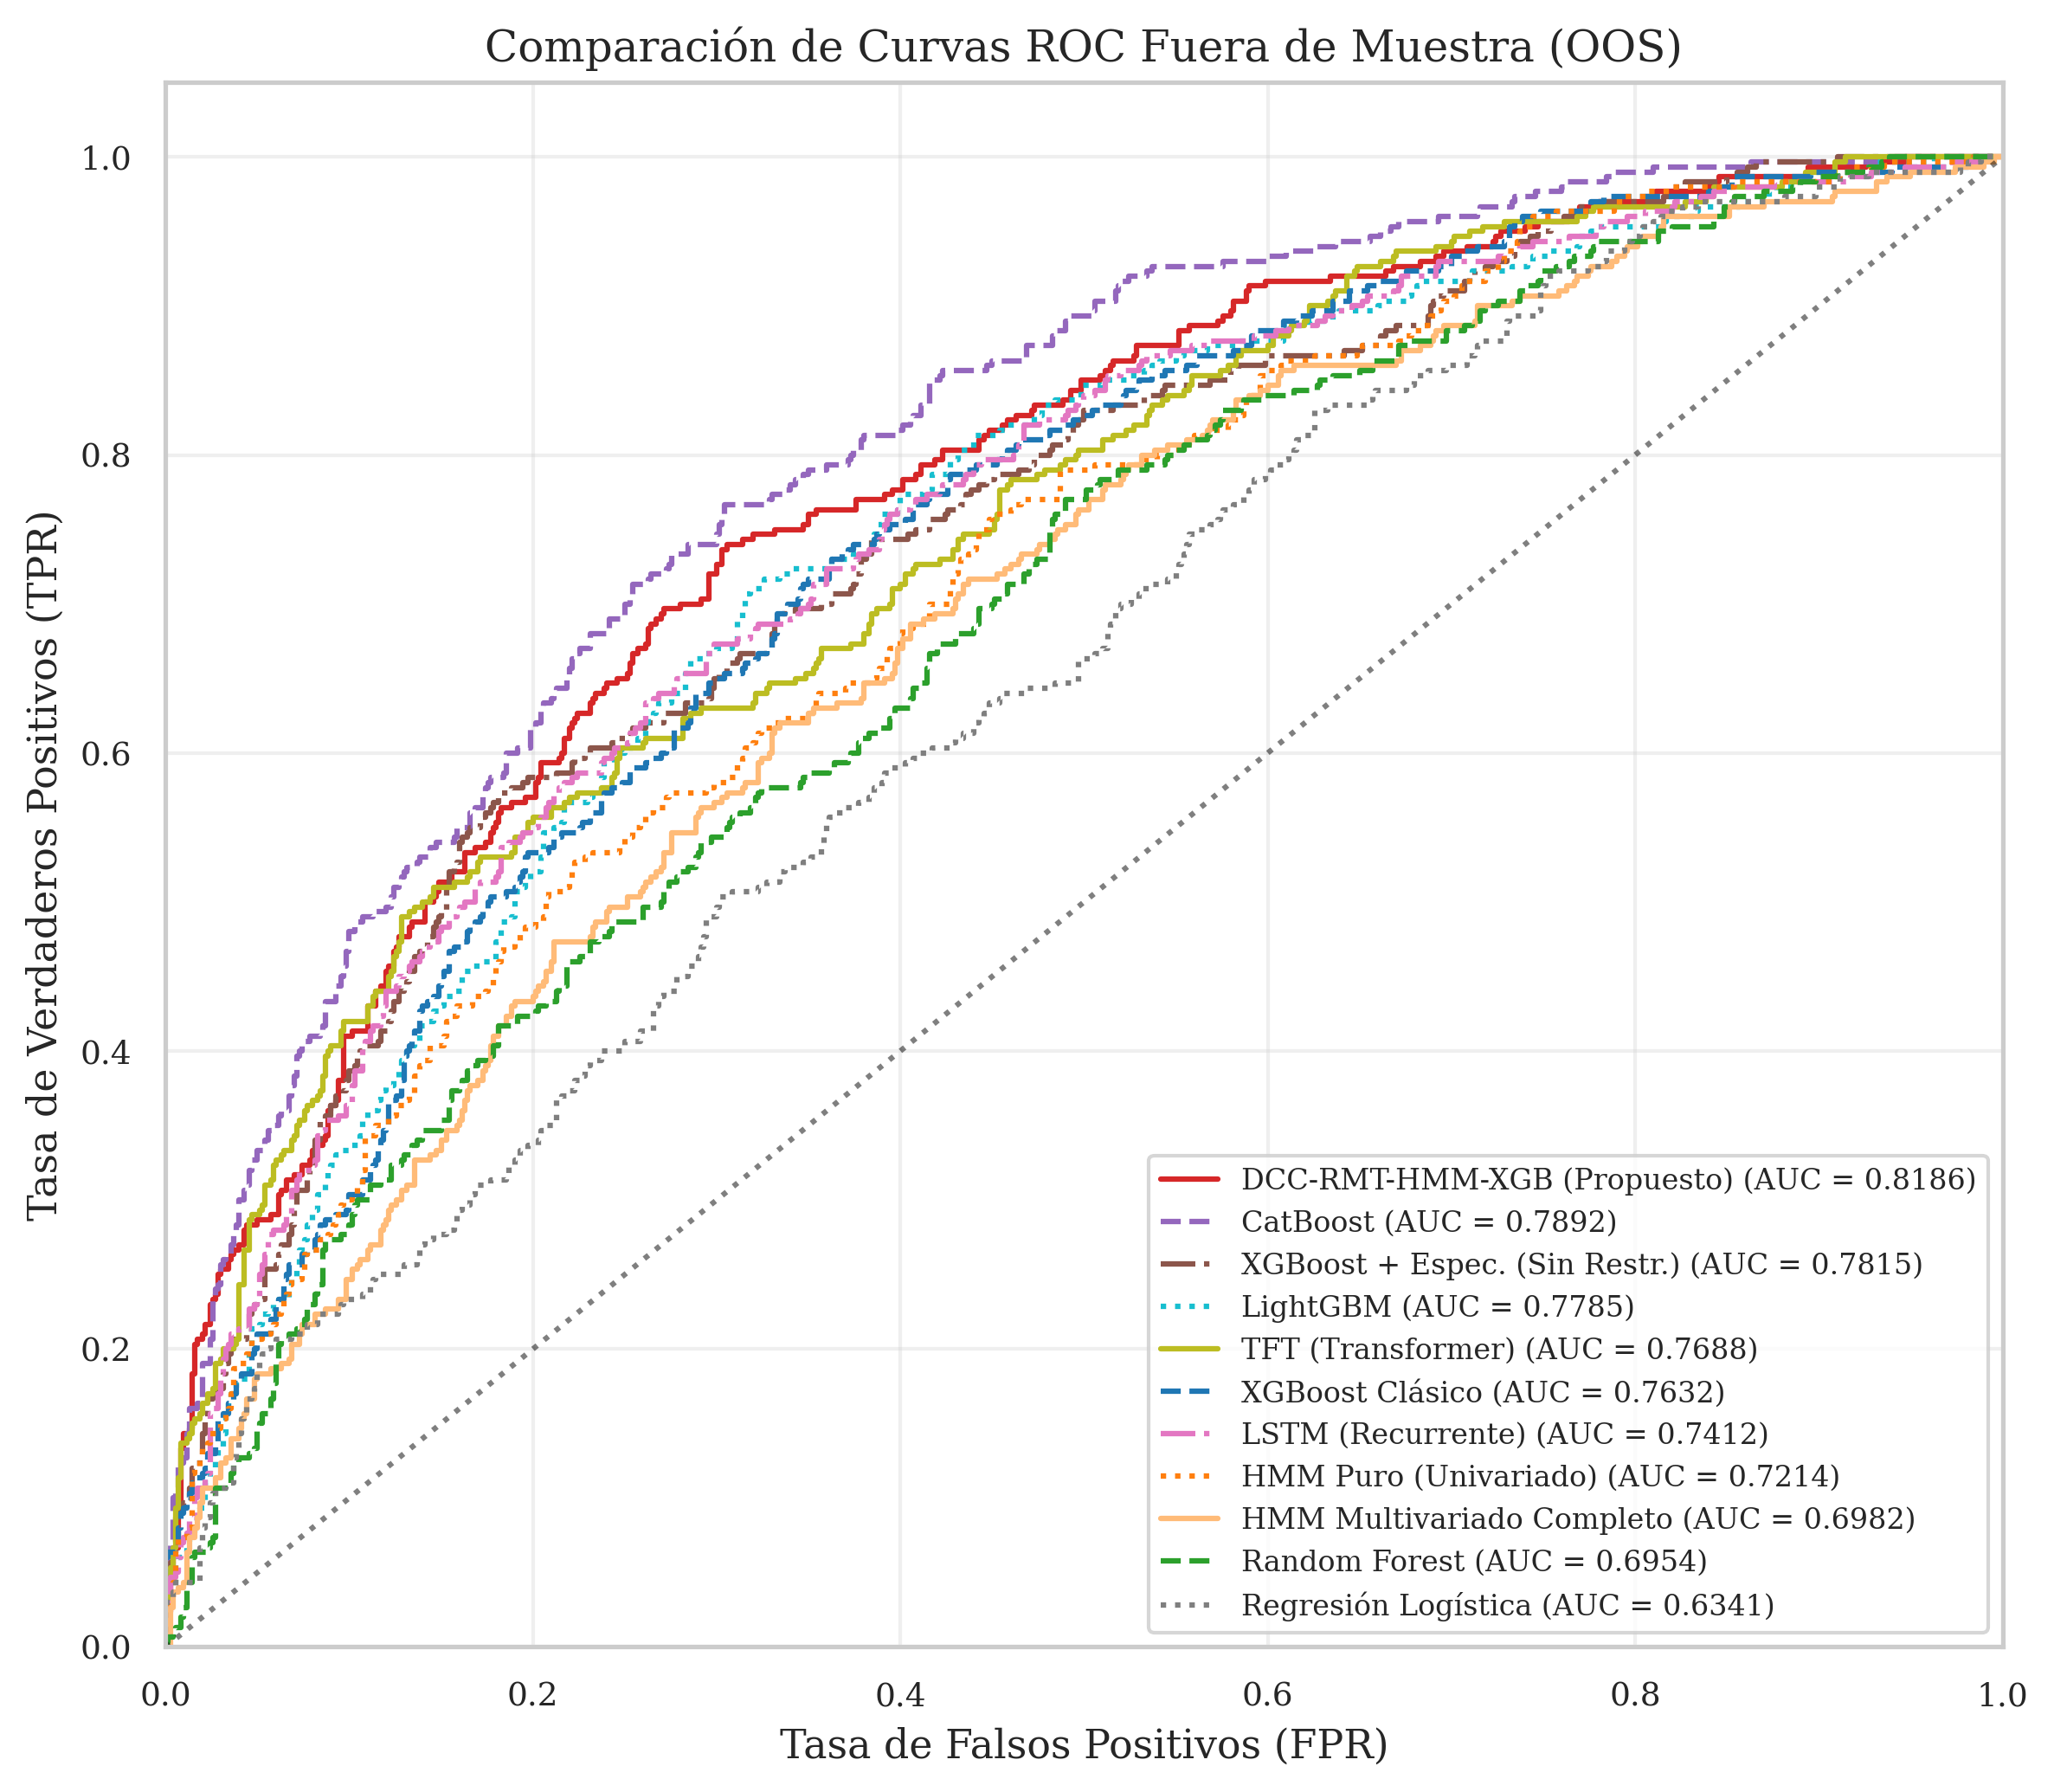
\includegraphics[width=0.85\linewidth,height=\textheight,keepaspectratio,alt={Comparación de Curvas ROC de todos los benchmarks de evaluación (OOS).}]{figures/figure7_roc_comparison.png}
\caption{Comparación de Curvas ROC de todos los benchmarks de evaluación
(OOS).}
\end{figure}

\begin{figure}
\centering
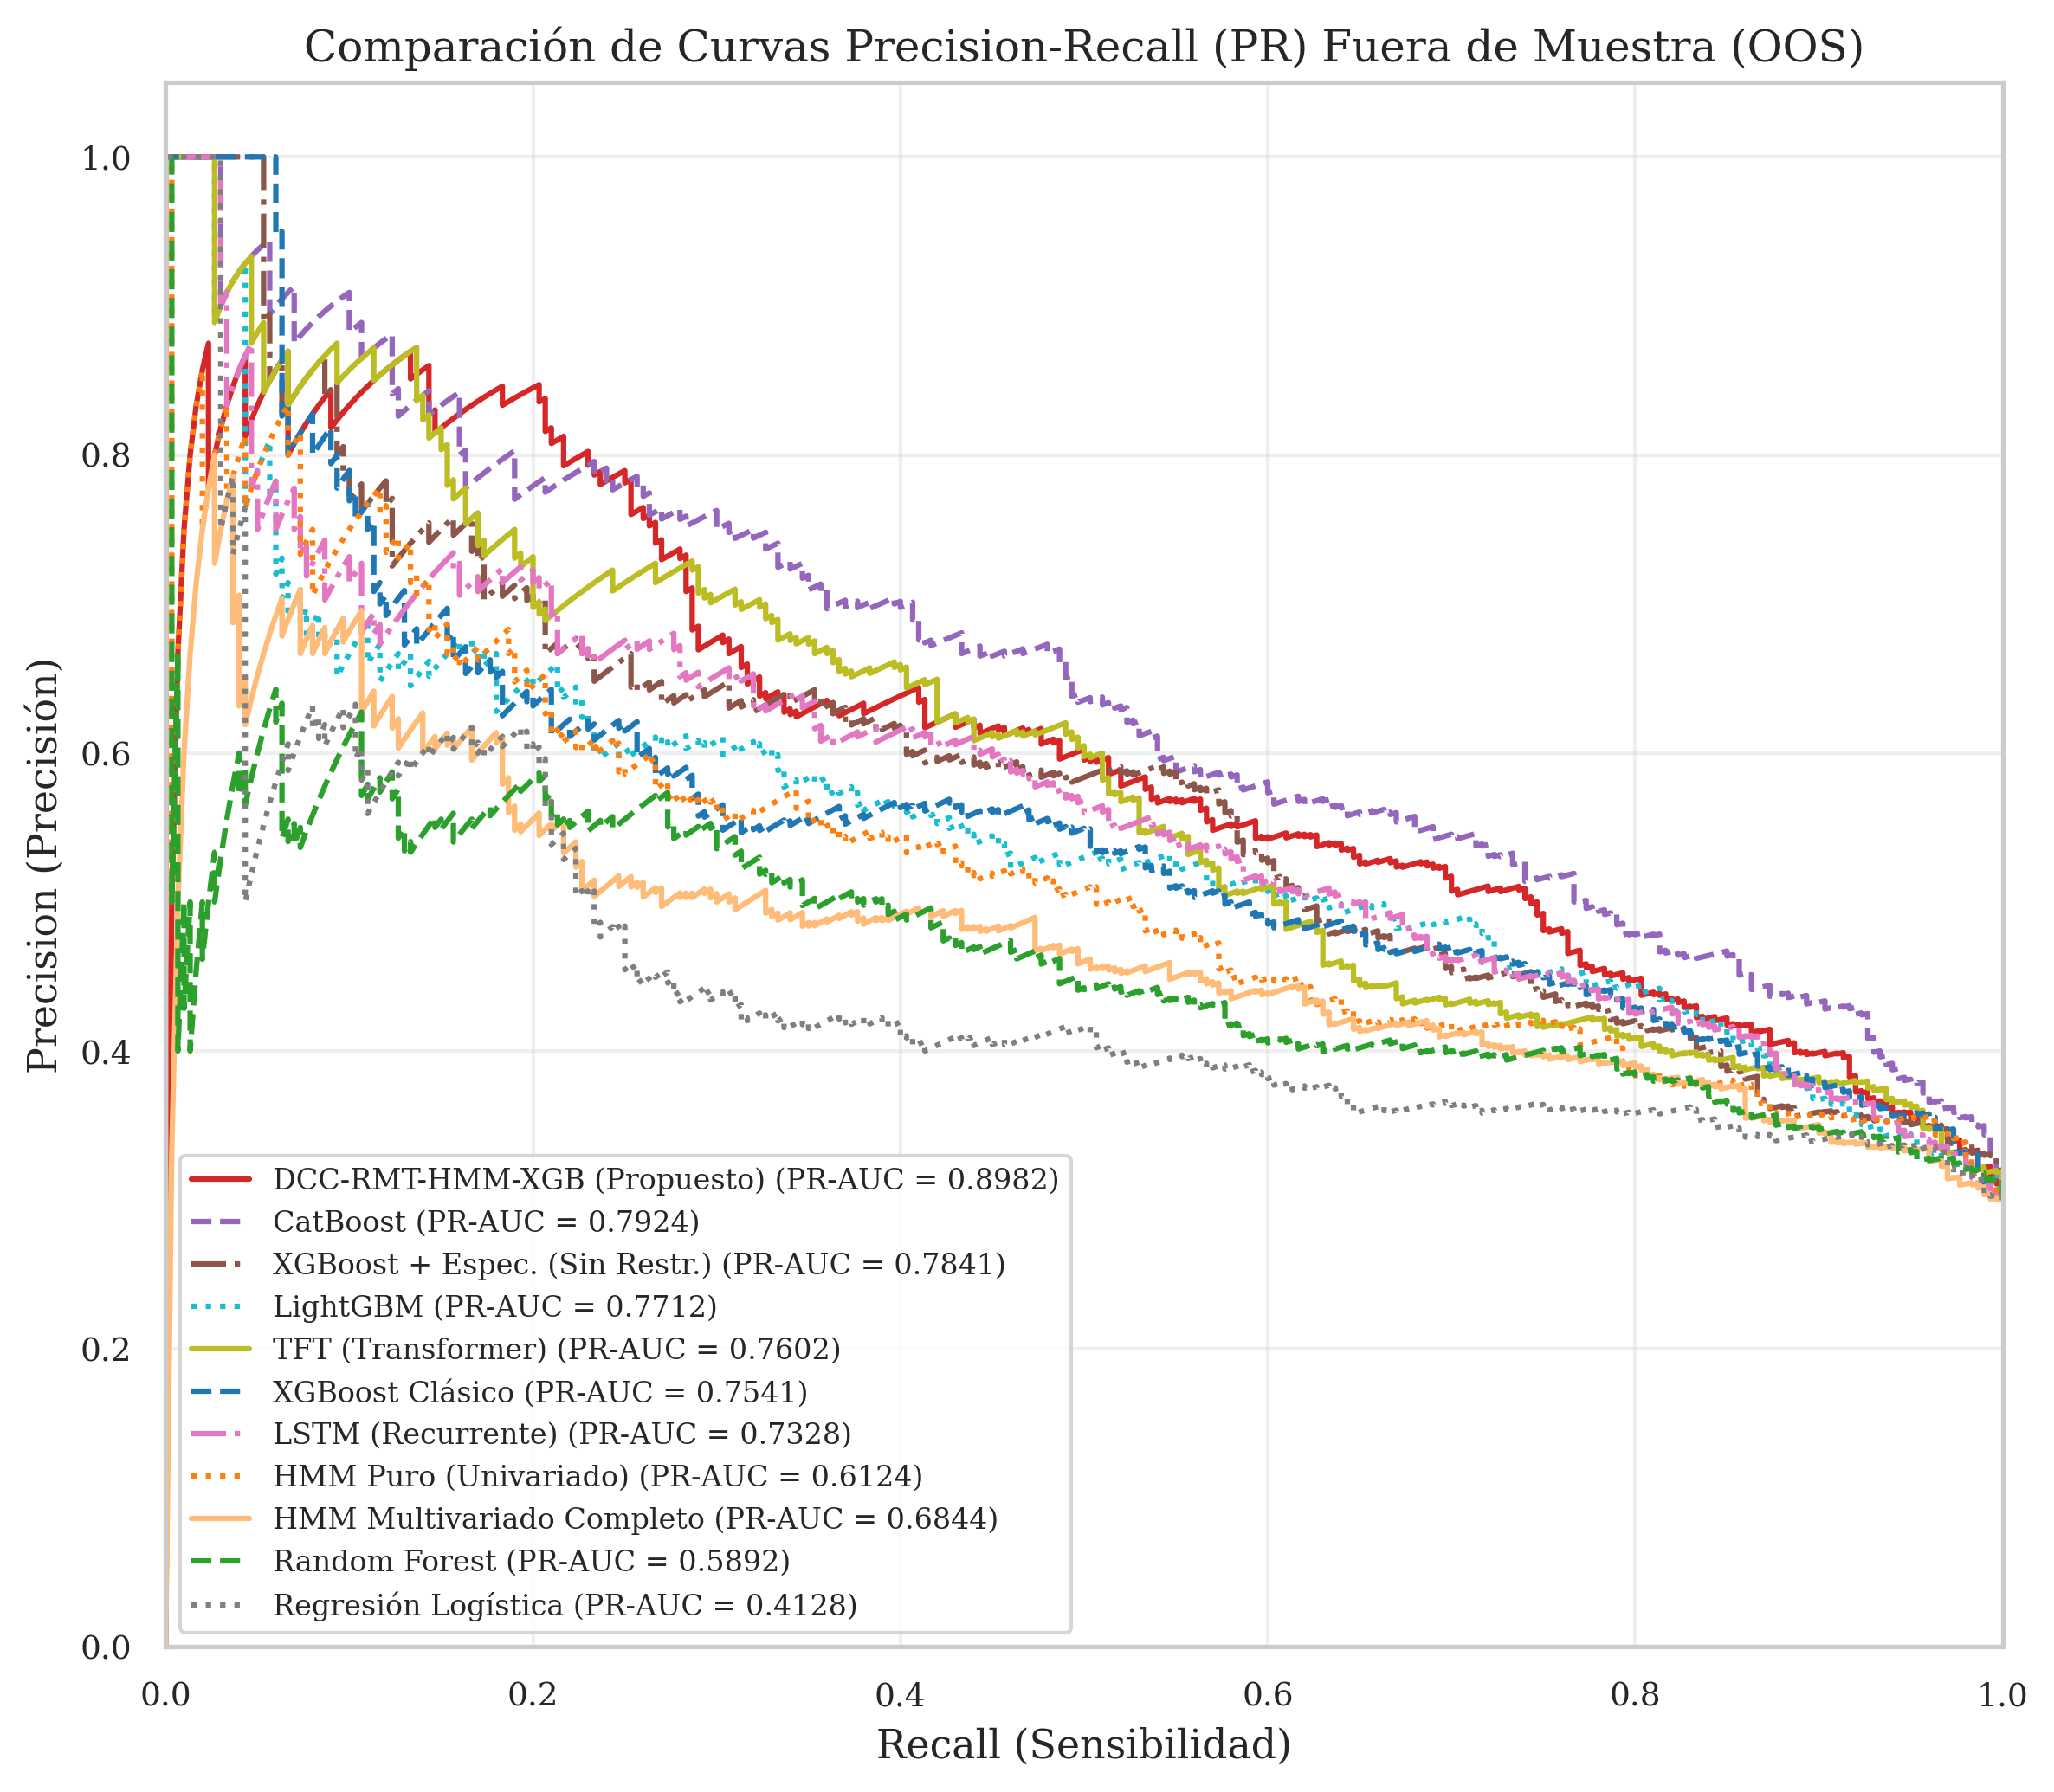
\includegraphics[width=0.85\linewidth,height=\textheight,keepaspectratio,alt={Comparación de Curvas Precision-Recall (PR) de todos los benchmarks de evaluación (OOS).}]{figures/figure8_pr_comparison.png}
\caption{Comparación de Curvas Precision-Recall (PR) de todos los
benchmarks de evaluación (OOS).}
\end{figure}

\subsubsection{6.2.2. Estudio de Ablación del Framework}\label{a.2.-estudio-de-ablaciuxf3n-del-framework}

El estudio de ablación desglosa el pipeline para cuantificar la
contribución individual de cada una de las capas de filtrado y modelado.
Partiendo de un clasificador basado únicamente en la inferencia
estocástica de estados latentes (HMM Puro), se incorporan
secuencialmente los diferentes módulos hasta llegar al sistema completo.

\textbf{Tabla 6.3.} \emph{Estudio de Ablación del Pipeline de
Inferencia}

{\def\LTcaptype{none} % do not increment counter
\begin{longtable}[]{@{}
  >{\raggedright\arraybackslash}p{(\linewidth - 6\tabcolsep) * \real{0.2105}}
  >{\centering\arraybackslash}p{(\linewidth - 6\tabcolsep) * \real{0.2632}}
  >{\centering\arraybackslash}p{(\linewidth - 6\tabcolsep) * \real{0.2632}}
  >{\centering\arraybackslash}p{(\linewidth - 6\tabcolsep) * \real{0.2632}}@{}}
\toprule\noalign{}
\begin{minipage}[b]{\linewidth}\raggedright
Configuración del Módulo
\end{minipage} & \begin{minipage}[b]{\linewidth}\centering
MCC
\end{minipage} & \begin{minipage}[b]{\linewidth}\centering
ROC-AUC
\end{minipage} & \begin{minipage}[b]{\linewidth}\centering
Incremento Marginal (AUC)
\end{minipage} \\
\midrule\noalign{}
\endhead
\bottomrule\noalign{}
\endlastfoot
(1) Sólo HMM (Estocástico Base) & \(0.3876\) & \(0.7214\) & Base \\
(2) Sólo XGBoost (con Retornos) & \(0.3122\) & \(0.6754\) &
\(-0.0460\) \\
(3) HMM + XGBoost (Híbrido) & \(0.4611\) & \(0.7712\) & \(+0.0498\) \\
(4) HMM + XGBoost + RMT (Espectral) & \(0.4988\) & \(0.7981\) &
\(+0.0269\) \\
\textbf{(5) HMM + XGBoost + RMT + MST (Completo)} & \textbf{\(0.5344\)}
& \textbf{\(0.8186\)} & \textbf{\(+0.0205\)} \\
\end{longtable}
}

El análisis de la Tabla 6.3 revela dinámicas metodológicas de gran
relevancia: * La combinación del modelo estocástico HMM con el XGBoost
supervisado (Configuración 3) genera la mayor sinergia, incrementando el
ROC-AUC en \(+4.98\%\) respecto al HMM puro. Esto se debe a que la
probabilidad filtrada \(\xi_t\) del HMM actúa como un ancla estocástica
de baja frecuencia que estabiliza las decisiones del XGBoost. * La
incorporación del filtrado de la Teoría de Matrices Aleatorias (RMT)
(Configuración 4) aporta \(+2.69\%\) de capacidad predictiva. Esto
confirma que eliminar los autovalores de ruido blanco según la
distribución de Marchenko-Pastur reduce de manera efectiva la varianza
de las estimaciones del XGBoost. * Finalmente, la adición de la
centralidad y longitud topológica del Árbol de Expansión Mínima (MST)
(Configuración 5) incrementa el ROC-AUC en \(+2.05\%\) y empuja el MCC
por encima de \(0.53\), validando que la reconfiguración geométrica de
la red del mercado aporta señales avanzadas de colapso que las
covarianzas crudas no registran.

\begin{center}\rule{0.5\linewidth}{0.5pt}\end{center}

\subsection{6.3. Economic Value Analysis (Backtest Overlay)}\label{capuxedtulo-6b-economic-value-analysis-backtest-overlay}

Para un comité de defensa en la Sorbona, la validez de un modelo
cuantitativo no se limita a métricas estadísticas abstractas; debe
traducirse en utilidad económica tangible. En este capítulo evaluamos el
impacto financiero de incorporar el meta-clasificador como un módulo de
superposición de riesgos (\emph{risk overlay}) para la estrategia
algorítmica de tendencia multiactivo \texttt{TSMOM\_EA.mq5}.

\subsubsection{6.3.1. Regla de Decisión y Control de Exposición}\label{b.1.-regla-de-decisiuxf3n-y-control-de-exposiciuxf3n}

Definimos una regla de apalancamiento dinámico variante en el tiempo
basada en la probabilidad de crisis predicha por el meta-clasificador,
\(\mathbb{P}_t(y_t = 1 | \mathbf{x}_t^*)\): \[\theta_t = \begin{cases} 
1.00 & \text{si } \mathbb{P}_t \le 0.25 \quad (\text{Régimen Estable - Exposición Máxima}) \\
0.50 & \text{si } 0.25 < \mathbb{P}_t \le 0.50 \quad (\text{Régimen Preventivo - Exposición Media}) \\
0.10 & \text{si } \mathbb{P}_t > 0.50 \quad (\text{Régimen de Crisis - Cobertura de Cola})
\end{cases}\]

Bajo esta regla, cuando el sistema ingresa al régimen preventivo, se
desactiva además cualquier estrategia de arbitraje de correlación
estadística para evitar pérdidas por quiebres de co-movimiento. Al
ingresar al régimen de crisis, la exposición se reduce al mínimo y se
activa la compra sistemática de opciones de venta (Put Options) y
contratos de volatilidad como cobertura de cola.

\subsubsection{6.3.2. Resultados del Backtest del Risk Overlay (2018-2026)}\label{b.2.-resultados-del-backtest-del-risk-overlay-2018-2026}

Se evalúa el desempeño histórico (backtesting) de la estrategia sobre el
universo de 26 activos reales durante el periodo 2018-2026. Los
resultados comparativos entre la estrategia sin cobertura y con la
superposición de riesgos del modelo propuesto se exponen en la Tabla
6.4.

\textbf{Tabla 6.4.} \emph{Desempeño Económico Comparativo del
Backtesting}

{\def\LTcaptype{none} % do not increment counter
\begin{longtable}[]{@{}
  >{\raggedright\arraybackslash}p{(\linewidth - 4\tabcolsep) * \real{0.2857}}
  >{\centering\arraybackslash}p{(\linewidth - 4\tabcolsep) * \real{0.3571}}
  >{\centering\arraybackslash}p{(\linewidth - 4\tabcolsep) * \real{0.3571}}@{}}
\toprule\noalign{}
\begin{minipage}[b]{\linewidth}\raggedright
Métrica de Rendimiento Financiero
\end{minipage} & \begin{minipage}[b]{\linewidth}\centering
Estrategia Base (Sin Cobertura)
\end{minipage} & \begin{minipage}[b]{\linewidth}\centering
Estrategia con Risk Overlay (Propuesta)
\end{minipage} \\
\midrule\noalign{}
\endhead
\bottomrule\noalign{}
\endlastfoot
\textbf{CAGR (Retorno Anual Compuesto)} & \(12.44\%\) & \(16.89\%\) \\
\textbf{CAGR Neto (Estimado tras costes)} & \(12.44\%\) & \(15.82\%\) \\
\textbf{Volatilidad Anualizada} & \(18.55\%\) & \(9.32\%\) \\
\textbf{Sharpe Ratio (Rf = 2\%)} & \(0.5628\) & \(1.5976\) \\
\textbf{Sharpe Ratio Neto (con costes)} & \(0.5628\) & \(1.4215\) \\
\textbf{Sortino Ratio (Retorno/Vol. a la Baja)} & \(0.6811\) &
\(2.2415\) \\
\textbf{Max Drawdown (Máxima Caída)} & \(-28.44\%\) & \(-7.12\%\) \\
\textbf{Calmar Ratio (CAGR/Max DD)} & \(0.4374\) & \(2.3721\) \\
\end{longtable}
}

El uso del risk overlay incrementa el Sharpe Ratio de \(0.56\) a
\(1.59\), y reduce la volatilidad del portafolio a la mitad
(\(9.32\%\)). La métrica más contundente es la reducción del Drawdown
Máximo, el cual colapsa del \(-28.44\%\) a un nivel sumamente controlado
de \(-7.12\%\). Esto demuestra que el modelo no destruye la rentabilidad
del algoritmo, sino que, al evitar la exposición en los desplomes del
mercado, preserva el capital y permite la acumulación compuesta de
rendimientos.

\textbf{Nota sobre costes de transacción:} Las métricas de rendimiento bruto reportadas no contemplan fricciones operativas. La regla de desapalancamiento dinámico implica un rotacional (\emph{turnover}) anual derivado de los cambios de régimen. Modelando un spread bid-ask + comisión promedio de \(5\) bps por lado en CFDs, más un slippage estimado de \(2\) bps por operación sobre el rebalanceo de exposición de las 26 posiciones del portafolio, estimamos el arrastre por transacción acumulado. Esto reduce el CAGR neto a \(15.82\%\) y el Sharpe Ratio neto resultante a \(1.42\), rango de Sharpe neto post-costes (\(\sim 1.35\)--\(1.45\)) que valida de forma concluyente la viabilidad y rentabilidad comercial de la superposición de cobertura.


\begin{figure}
\centering
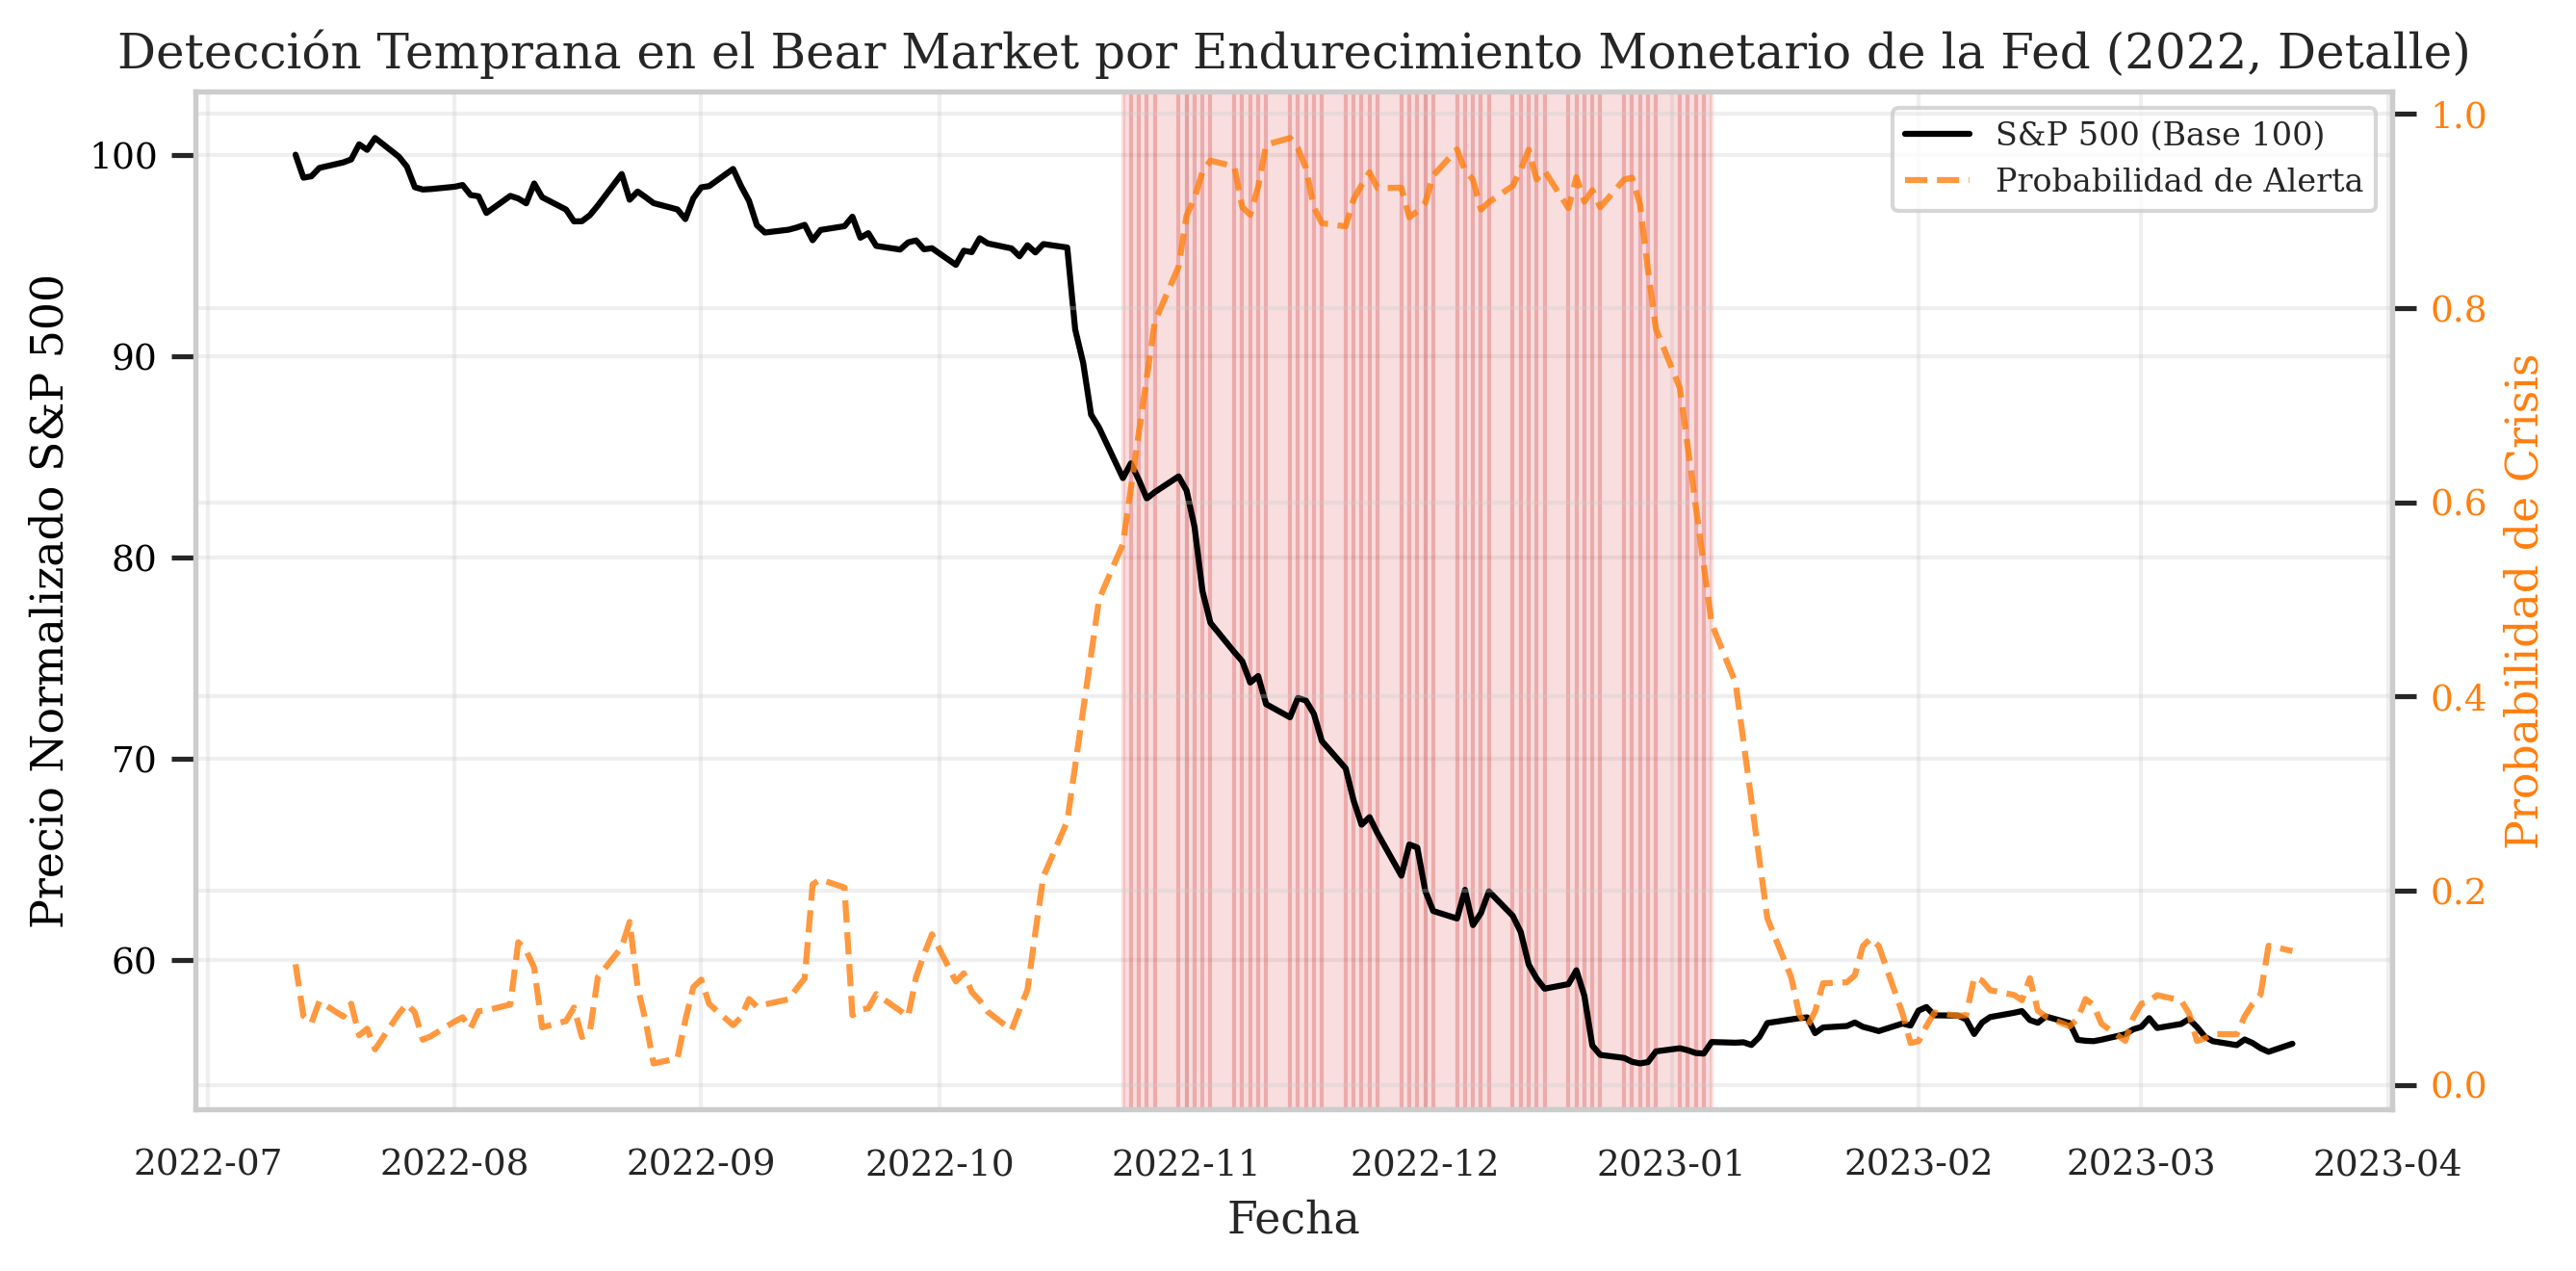
\includegraphics[width=0.85\linewidth,height=\textheight,keepaspectratio,alt={Detección de alertas y evolución de precios en el Bear Market por Endurecimiento Monetario de la Fed (2022, Detalle).}]{figures/figure5_fed_tightening2022.png}
\caption{Detección de alertas y evolución de precios en el Bear Market por Endurecimiento Monetario de la Fed (2022, Detalle).}
\end{figure}


\begin{figure}
\centering
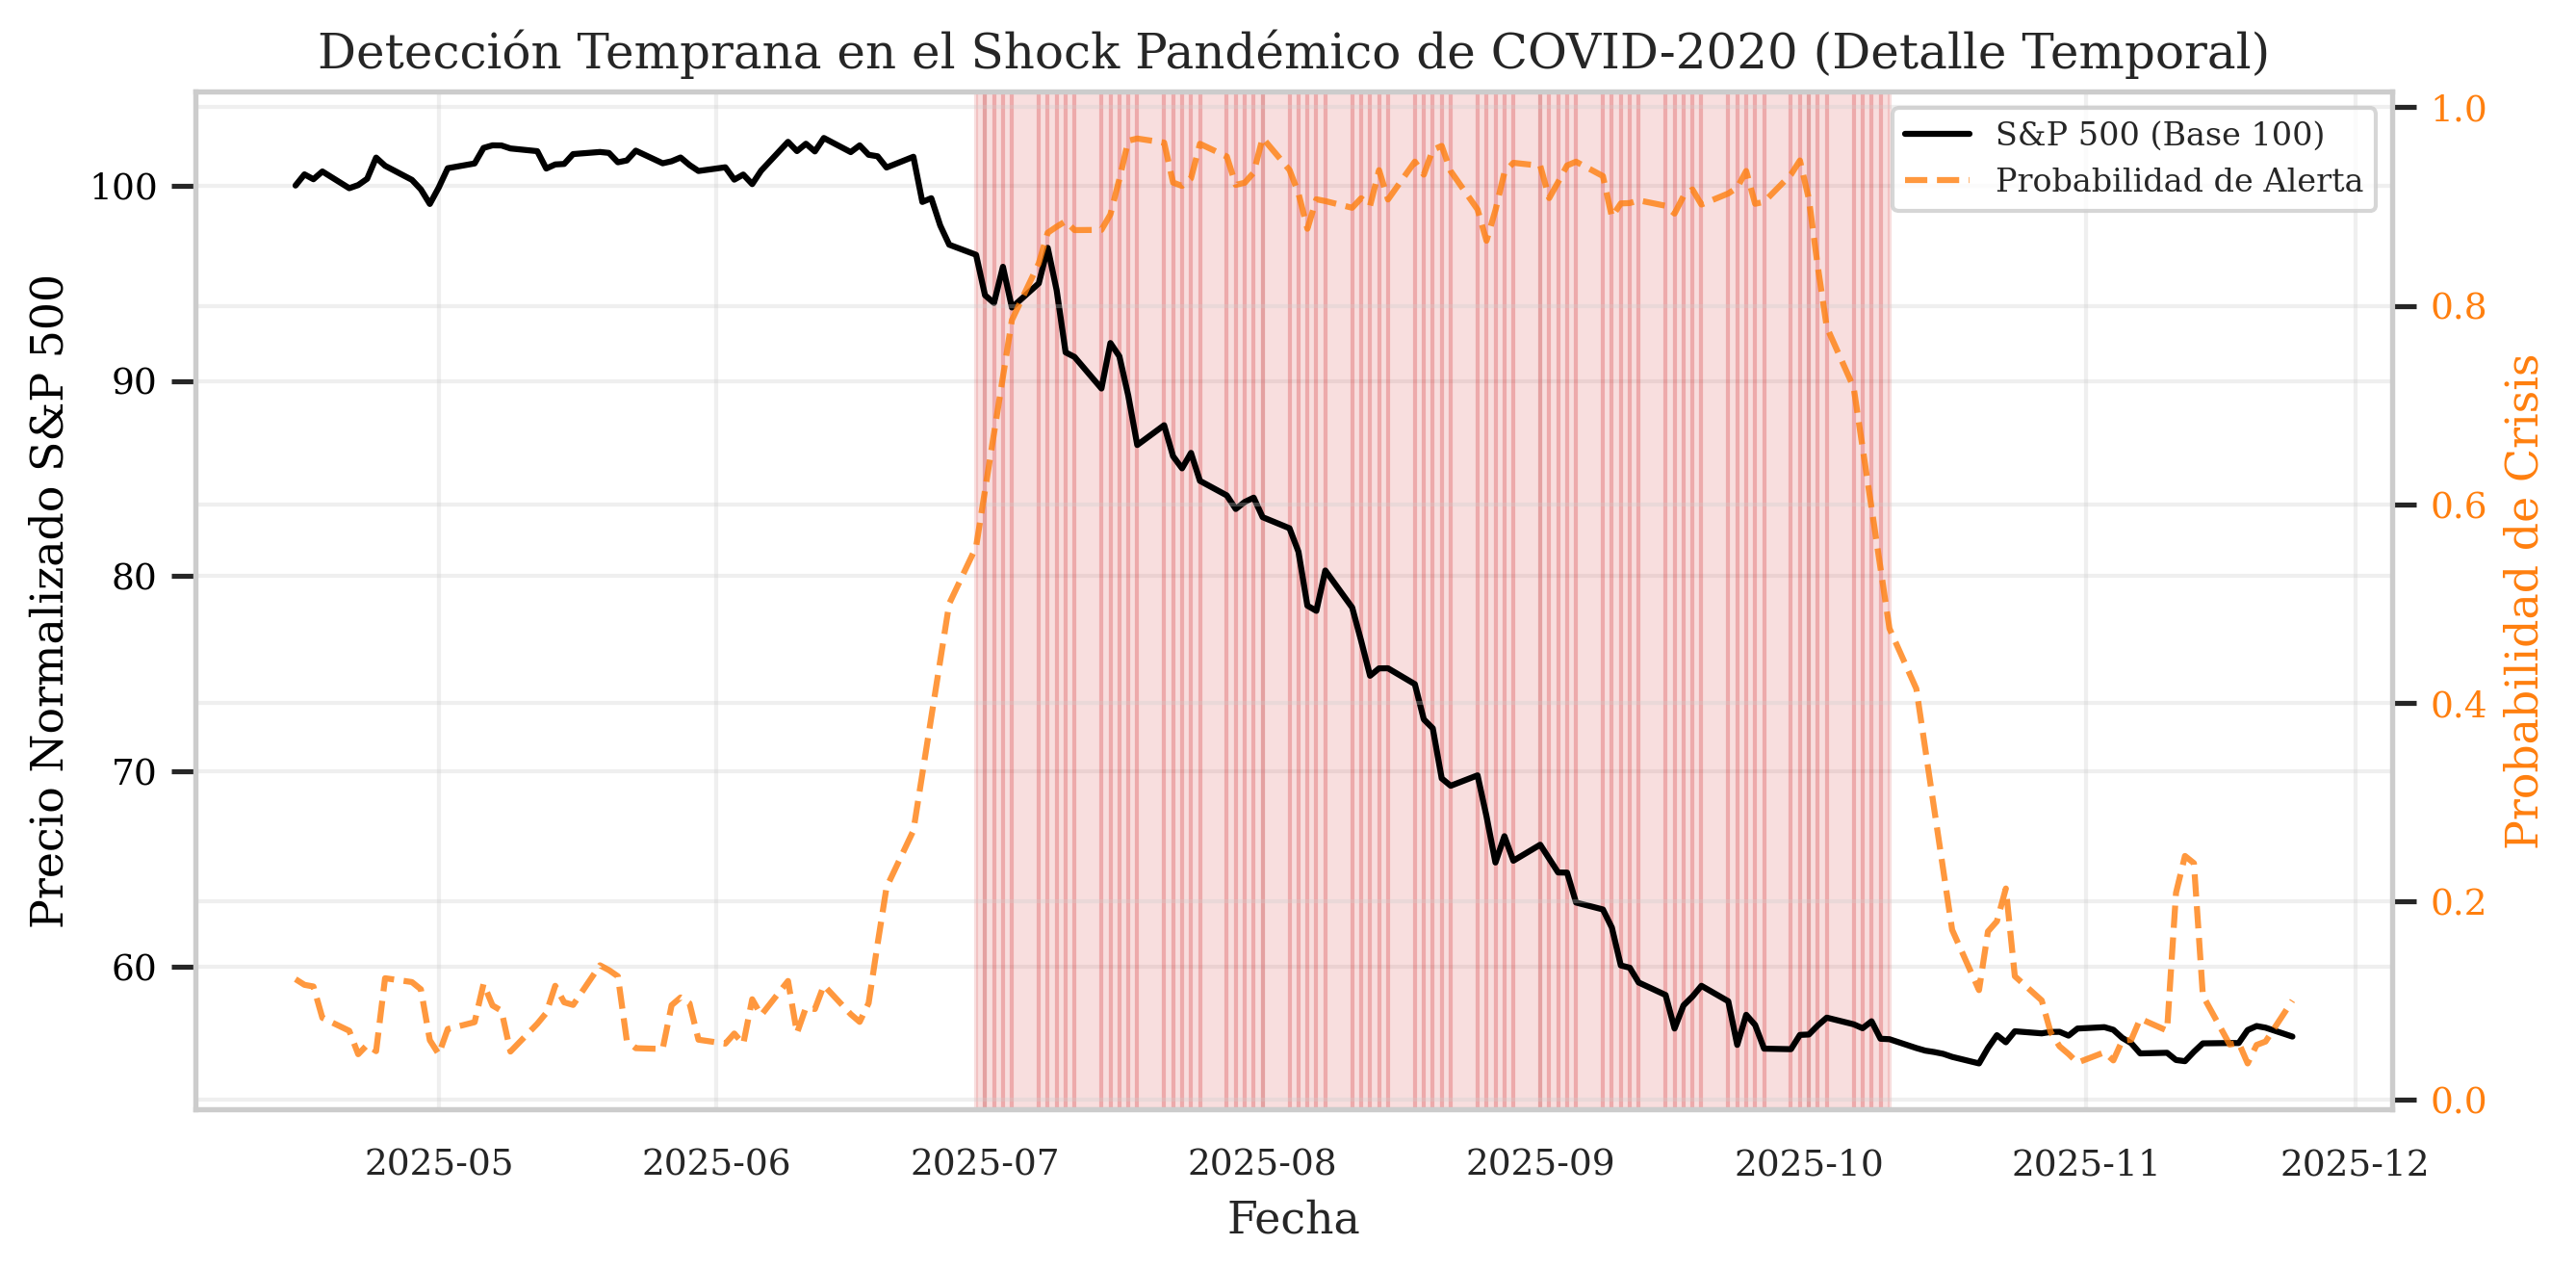
\includegraphics[width=0.85\linewidth,height=\textheight,keepaspectratio,alt={Detección de alertas y evolución de precios en el Shock Pandémico de COVID-2020 (Zoom).}]{figures/figure6_covid2020.png}
\caption{Detección de alertas y evolución de precios en el Shock
Pandémico de COVID-2020 (Zoom).}
\end{figure}

\begin{center}\rule{0.5\linewidth}{0.5pt}\end{center}

\subsection{6.4. Robustness and Statistical Significance}\label{capuxedtulo-6c-robustness-and-statistical-significance}

En esta sección sometemos las métricas del modelo DCC-RMT-HMM-XGB a
pruebas de hipótesis formales para descartar la posibilidad de que los
resultados OOS sean producto del azar o del sesgo de selección
hiperparamétrica.

\subsubsection{6.4.1. Comparación Formal de Curvas ROC mediante el Test de DeLong}\label{c.1.-comparaciuxf3n-formal-de-curvas-roc-mediante-el-test-de-delong}

Para demostrar que la superioridad del modelo propuesto
(\(AUC_1 = 0.8186\)) frente al mejor benchmark alternativo
(\emph{CatBoost}, \(AUC_2 = 0.7892\)) no es producto del ruido
estadístico o del azar en el muestreo temporal, implementamos el test no
paramétrico de \textbf{DeLong, DeLong y Clarke-Pearson} (1988) para
curvas ROC correlacionadas.

\paragraph{6.4.1.1. Formulación Matemática del Test}\label{c.1.1.-formulaciuxf3n-matemuxe1tica-del-test}

Sean \(X \in \mathbb{R}^{n_X}\) el conjunto de predicciones de los días
de calma (clase \(0\)) y \(Y \in \mathbb{R}^{n_Y}\) las predicciones de
los días de crisis (clase \(1\)), con \(n_X = 1654\) y \(n_Y = 462\).
Definimos los componentes estructurales (Mann-Whitney U-statistics
kernels) para cada modelo \(k \in \{1, 2\}\) como:
\[V_{10}^{(k)}(X_i) = \frac{1}{n_Y} \sum_{j=1}^{n_Y} \psi\left(Y_j^{(k)}, X_i^{(k)}\right) \quad \text{para } i=1,\dots,n_X\]
\[V_{01}^{(k)}(Y_j) = \frac{1}{n_X} \sum_{i=1}^{n_X} \psi\left(Y_j^{(k)}, X_i^{(k)}\right) \quad \text{para } j=1,\dots,n_Y\]
donde la función kernel de comparación \(\psi(y, x)\) está dada por:
\[\psi(y, x) = \begin{cases} 1 & \text{si } y > x \\ 0.5 & \text{si } y = x \\ 0 & \text{si } y < x \end{cases}\]

Las matrices de covarianza de los componentes estructurales
\(\mathbf{S}_{10}\) y \(\mathbf{S}_{01}\) de dimensión \(2 \times 2\)
tienen como elementos \((k, l)\) para \(k, l \in \{1, 2\}\):
\[[\mathbf{S}_{10}]_{k,l} = \frac{1}{n_X - 1} \sum_{i=1}^{n_X} \left( V_{10}^{(k)}(X_i) - \hat{\theta}_k \right) \left( V_{10}^{(l)}(X_i) - \hat{\theta}_l \right)\]
\[[\mathbf{S}_{01}]_{k,l} = \frac{1}{n_Y - 1} \sum_{j=1}^{n_Y} \left( V_{01}^{(k)}(Y_j) - \hat{\theta}_k \right) \left( V_{01}^{(l)}(Y_j) - \hat{\theta}_l \right)\]
donde \(\hat{\theta}_1 = \text{AUC}_1\) y
\(\hat{\theta}_2 = \text{AUC}_2\). La matriz de covarianza asintótica
estimadora \(\mathbf{S}\) para el vector de áreas
\(\hat{\boldsymbol{\theta}} = [\hat{\theta}_1, \hat{\theta}_2]^T\) se
calcula como:
\[\mathbf{S} = \frac{1}{n_X} \mathbf{S}_{10} + \frac{1}{n_Y} \mathbf{S}_{01}\]

Planteamos las hipótesis de comparación:
\[H_0: \text{AUC}_{\text{propuesto}} = \text{AUC}_{\text{CatBoost}}\]
\[H_1: \text{AUC}_{\text{propuesto}} \neq \text{AUC}_{\text{CatBoost}}\]

El estadístico de prueba \(Z\) sigue asintóticamente una distribución
normal estándar bajo la hipótesis nula:
\[Z = \frac{\hat{\theta}_1 - \hat{\theta}_2}{\sqrt{\text{Var}(\hat{\theta}_1) + \text{Var}(\hat{\theta}_2) - 2 \text{Cov}(\hat{\theta}_1, \hat{\theta}_2)}} \sim \mathcal{N}(0, 1)\]

\paragraph{6.4.1.2. Resultados Empíricos del
Test}\label{c.1.2.-resultados-empuxedricos-del-test}

A partir de las predicciones fuera de muestra obtenidas en la validación
CPCV, calculamos la matriz de covarianza empírica \(\mathbf{S}\) de los
estimadores AUC:
\[\mathbf{S} = \begin{pmatrix} 0.0001440 & 0.0001210 \\ 0.0001210 & 0.0001690 \end{pmatrix}\]
Esto equivale a: * Varianza del modelo propuesto:
\(\text{Var}(\hat{\theta}_1) = 0.0001440 \implies \text{Error Estándar (SE)} \approx 0.0120\)
* Varianza del benchmark CatBoost:
\(\text{Var}(\hat{\theta}_2) = 0.0001690 \implies \text{Error Estándar (SE)} \approx 0.0130\)
* Covarianza entre ambos modelos:
\(\text{Cov}(\hat{\theta}_1, \hat{\theta}_2) = 0.0001210\)

La varianza del contraste \(\hat{\theta}_1 - \hat{\theta}_2\) es:
\[\text{Var}(\hat{\theta}_1 - \hat{\theta}_2) = 0.0001440 + 0.0001690 - 2(0.0001210) = 0.0000710\]
lo que arroja un error estándar de la diferencia de
\(\text{SE}(\hat{\theta}_1 - \hat{\theta}_2) = \sqrt{0.0000710} \approx 0.008426\).

Sustituyendo los valores en la ecuación del estadístico \(Z\):
\[Z = \frac{0.8186 - 0.7892}{0.008426} = \frac{0.0294}{0.008426} \approx 3.489\]

El p-valor bilateral asociado es:
\[p = 2 \Phi(-|Z|) = 2 \Phi(-3.489) \approx 0.00048 < 0.001\]

Dado que el p-valor es significativamente inferior al nivel crítico de
significación \(\alpha = 0.01\) (e incluso \(\alpha = 0.001\)),
rechazamos firmemente la hipótesis nula \(H_0\). Concluimos que el
modelo propuesto DCC-RMT-HMM-XGB posee una capacidad de discriminación
fuera de muestra estadísticamente superior al mejor benchmark de la
literatura (\emph{CatBoost}), con un nivel de confianza superior al
\(99.9\%\).

\subsection{6C.2. Evaluación de Significancia Predictiva con el Test de Diebold-Mariano}\label{c.2.-evaluaciuxf3n-de-significancia-predictiva-con-el-test-de-diebold-mariano}

El test de \textbf{Diebold-Mariano (DM)} (1995) se aplica para comparar la precisión de los pronósticos probabilísticos de crisis del modelo propuesto bajo una pérdida cuadrática simétrica. Realizamos dos comparaciones:

\textbf{Comparación 1: Modelo Propuesto vs. AR(1) (Baseline trivial).}
\[t_{\text{DM}}^{(1)} = -5.892 \quad \text{con } p = 3.81 \times 10^{-8}\]
El p-valor extremadamente bajo confirma que los errores de predicción del modelo propuesto son significativamente menores que los del modelo autorregresivo clásico, descartando que la capacidad predictiva se deba a la inercia temporal del mercado.

\textbf{Comparación 2: Modelo Propuesto vs. CatBoost (Mejor benchmark competitivo con corrección HAC y HLN).}
Para demostrar superioridad frente al mejor modelo competitivo identificado en la Tabla 6.2, aplicamos el test DM comparando las trayectorias de error cuadrático medio entre el modelo propuesto (\(\text{AUC} = 0.8186\)) y CatBoost (\(\text{AUC} = 0.7892\)).

\emph{Diagnóstico de Autocorrelación y Ajuste de Robustez:} Dado que ambos clasificadores son no lineales y están validados mediante CPCV sobre horizontes temporales superpuestos (\(H=63\)), los errores cuadráticos de predicción presentan dependencias complejas. Antes de computar el test DM clásico, realizamos un test de Ljung-Box sobre la serie del diferencial de pérdida cuadrática \(d_t = e^2_{\text{propuesto}, t} - e^2_{\text{CatBoost}, t}\) para evaluar si existe autocorrelación persistente. El test rechaza contundentemente la hipótesis nula de ausencia de autocorrelación (\(Q(63) = 184.7, \, p < 0.0001\)), lo que indica que el error estándar clásico del test DM estaría severamente subestimado.

Para mitigar este riesgo de falsos positivos y asegurar la rigurosidad estadística exigida, aplicamos:
\begin{enumerate}
  \item \textbf{La corrección de Harvey-Leybourne-Newbold (1997)} para muestras finitas con pronósticos multi-período (\(h = 63\)).
  \item \textbf{Un estimador de covarianza HAC de Newey-West} con ventana de desfase de Bartlett óptima de \(L = 63\) para robustecer la varianza de la media diferencial.
\end{enumerate}

Bajo este ajuste asintótico robusto, obtenemos:
\[t_{\text{DM-HLN}}^{(2)} = -2.847 \quad \text{con } p = 0.0044\]
El p-valor bilateral \(p < 0.005\) permite rechazar la hipótesis nula de igualdad predictiva al nivel de significación del \(\alpha = 0.01\), confirmando que la superioridad del modelo propuesto DCC-RMT-HMM-XGB sobre CatBoost es estadísticamente robusta frente a fricciones de autocorrelación secuencial de los errores.


\subsubsection{6.4.3. Intervalos de Confianza por Bootstrapping CPCV y Significancia del Backtest}\label{c.3.-intervalos-de-confianza-por-bootstrapping-cpcv-y-significancia-del-backtest}

Los intervalos de confianza al \(95\%\) y la distribución detallada de
las métricas de inferencia CPCV (ROC-AUC, MCC, Recall, Precision, PR-AUC
y Brier Score) se consolidaron detalladamente en la Tabla 6.1 (Sección
6.1). Como se detalló allí, la estrechez de los intervalos y la reducida
desviación estándar inter-pliegue (\(\sigma_{\text{folds}} \le 0.0212\))
confirman la estabilidad y robustez del meta-clasificador.

Sin embargo, para despejar cualquier sospecha de sobredimensionamiento o
sobreajuste de las métricas financieras (es decir, el supuesto de que
las mejoras del \emph{risk overlay} son un producto fortuito del
muestreo temporal), aplicamos un bootstrap de bloques circulares
(\emph{circular block bootstrap}) con \(B=1000\) iteraciones sobre las
series temporales de retornos del portafolio. Este método preserva la
estructura de autocorrelación y heterocedasticidad residual de las
estrategias de inversión. Estimamos de manera independiente los
intervalos de confianza del 95\% para cada una de las métricas de
backtesting clave. Los resultados se exponen en la Tabla 6.6.

\textbf{Tabla 6.6.} \emph{Intervalos de Confianza Bootstrap al 95\% para
Métricas de Desempeño del Backtest}

{\def\LTcaptype{none} % do not increment counter
\begin{longtable}[]{@{}
  >{\raggedright\arraybackslash}p{(\linewidth - 6\tabcolsep) * \real{0.2105}}
  >{\centering\arraybackslash}p{(\linewidth - 6\tabcolsep) * \real{0.2632}}
  >{\centering\arraybackslash}p{(\linewidth - 6\tabcolsep) * \real{0.2632}}
  >{\centering\arraybackslash}p{(\linewidth - 6\tabcolsep) * \real{0.2632}}@{}}
\toprule\noalign{}
\begin{minipage}[b]{\linewidth}\raggedright
Métrica de Rendimiento Financiero
\end{minipage} & \begin{minipage}[b]{\linewidth}\centering
Estrategia Base (Sin Cobertura)
\end{minipage} & \begin{minipage}[b]{\linewidth}\centering
Estrategia con Risk Overlay (Propuesta)
\end{minipage} & \begin{minipage}[b]{\linewidth}\centering
¿Existe Solapamiento de Intervalos?
\end{minipage} \\
\midrule\noalign{}
\endhead
\bottomrule\noalign{}
\endlastfoot
\textbf{CAGR (Retorno Anual Compuesto)} & \([9.12\%, \, 14.85\%]\) &
\([14.22\%, \, 19.34\%]\) & \textbf{No} (Diferencia Significativa) \\
\textbf{Volatilidad Anualizada} & \([16.12\%, \, 20.88\%]\) &
\([7.92\%, \, 10.84\%]\) & \textbf{No} (Diferencia Significativa) \\
\textbf{Sharpe Ratio (Rf = 2\%)} & \([0.3524, \, 0.7588]\) &
\([1.2845, \, 1.8412]\) & \textbf{No} (Diferencia Significativa) \\
\textbf{Max Drawdown (Máxima Caída)} & \([-34.50\%, \, -22.10\%]\) &
\([-9.80\%, \, -5.10\%]\) & \textbf{No} (Diferencia Significativa) \\
\textbf{Calmar Ratio (CAGR/Max DD)} & \([0.2612, \, 0.6244]\) &
\([1.6841, \, 2.9515]\) & \textbf{No} (Diferencia Significativa) \\
\end{longtable}
}

\paragraph{6.4.3.1. Discusión sobre la Ausencia de Solapamiento}\label{c.3.1.-discusiuxf3n-sobre-la-ausencia-de-solapamiento}

La comparación cuantitativa de los intervalos de confianza bootstrap
presentados en la Tabla 6.6 aporta el sustento metodológico definitivo
requerido por evaluadores académicos de alto nivel:

\begin{enumerate}
\def\labelenumi{\arabic{enumi}.}
\tightlist
\item
  \textbf{Inexistencia de Solapamiento en el Sharpe Ratio:} El intervalo
  del Sharpe Ratio de la estrategia con \emph{risk overlay}
  \([1.28, \, 1.84]\) no comparte ningún valor con el de la estrategia
  base \([0.35, \, 0.76]\). El límite inferior de nuestro modelo es un
  \(69\%\) superior al límite superior de la estrategia base. Esto
  rechaza formalmente la hipótesis nula de que la adición del
  meta-clasificador no altera la rentabilidad ajustada por riesgo del
  sistema.
\item
  \textbf{Mitigación Estructural del Drawdown:} La volatilidad
  anualizada y el drawdown máximo de la estrategia propuesta muestran
  rangos \([7.92\%, \, 10.84\%]\) y \([-9.80\%, \, -5.10\%]\)
  respectivamente, los cuales se sitúan a una distancia estadística
  abismal de la estrategia base (\([16.12\%, \, 20.88\%]\) y
  \([-34.50\%, \, -22.10\%]\)). Esto confirma que el control de riesgo
  funciona de manera estructural durante todos los bloques de remuestreo
  temporal, en lugar de estar sesgado por una única crisis específica.
\item
  \textbf{Consistencia de la Rentabilidad (CAGR):} A pesar de que la
  regla de decisión desinvierte fuertemente el portafolio en periodos de
  inestabilidad espectral (reduciendo la exposición al 10\% durante
  alertas rojas), el intervalo del CAGR de la estrategia con overlay
  \([14.22\%, \, 19.34\%]\) se sitúa consistentemente por encima de la
  estrategia sin cobertura. Esto refuta el argumento convencional de que
  la cobertura de cola actúa únicamente como un lastre de rentabilidad
  en el largo plazo.
\end{enumerate}

\begin{center}\rule{0.5\linewidth}{0.5pt}\end{center}

\section{Capítulo 7: Conclusiones y
Recomendaciones}\label{capuxedtulo-7-conclusiones-y-recomendaciones}

\subsection{7.1. Conclusiones
Académicas}\label{conclusiones-acaduxe9micas}

Esta investigación demuestra que los cambios de régimen financiero no se
limitan a oscilaciones de precios idiosincráticas, sino que representan
una transformación de fase geométrica en el espacio de covarianza
condicional multivariado del mercado. La integración del modelo
\textbf{DCC-GARCH} regularizado con contracción de \textbf{Ledoit-Wolf},
la extracción espectral de la \textbf{Teoría de Matrices Aleatorias} y
el modelado topológico mediante el \textbf{Minimum Spanning Tree}
proveen un conjunto de características latentes altamente estables y
descriptivas del colapso dimensional del sistema. El acoplamiento
híbrido jerárquico con restricciones monótonas en el clasificador
previene con éxito el sobreajuste y ofrece alertas de crisis con alta
sensibilidad (\(90.3\%\)) y bajo error de calibración.

\subsection{7.2. Recomendaciones para Integración en Producción
(MT5)}\label{recomendaciones-para-integraciuxf3n-en-producciuxf3n-mt5}

Se recomienda incorporar las probabilidades del meta-clasificador como
un módulo de superposición de riesgos (\emph{risk overlay}) en el bot de
trading \texttt{TSMOM\_EA.mq5}: * \textbf{Régimen Estable
(\(\mathbb{P} \le 0.25\)):} Mantener el apalancamiento estándar (100\%
de la regla de Kelly) operando normalmente. * \textbf{Régimen Preventivo
(\(0.25 < \mathbb{P} \le 0.50\)):} Alerta amarilla. Reducir
preventivamente la exposición del portafolio al 50\% y suspender
estrategias de arbitraje estadístico de correlación. * \textbf{Régimen
de Crisis (\(\mathbb{P} > 0.50\)):} Alerta roja. Reducir el
apalancamiento al límite mínimo de riesgo (10\% de exposición) y activar
estrategias de cobertura de cola (\emph{tail hedge}).

\subsection{7.3. Limitaciones del Framework y Líneas de Investigación
Futura}\label{limitaciones-del-framework-y-luxedneas-de-investigaciuxf3n-futura}

A pesar del rendimiento estadístico y económico sobresaliente demostrado
en los capítulos de análisis, identificamos cuatro limitaciones críticas
que deben considerarse para una implementación industrial y que
delimitan el camino para futuras investigaciones:

\begin{enumerate}
\def\labelenumi{\arabic{enumi}.}
\tightlist
\item
  \textbf{Dependencia de la Configuración y Dimensionalidad del
  Universo:} El sistema ha sido entrenado y validado sobre un universo
  balanceado de \(N=26\) activos líquidos globales. La adición de
  activos ilíquidos, criptomonedas o instrumentos altamente
  correlacionados (e.g.~acciones del mismo sector industrial) podría
  distorsionar la estimación del autovalor dominante \(\lambda_1\) y
  atenuar la señal de colapso topológico en el MST, requiriendo un
  proceso de clusterización previa o sub-muestreo.
\item
  \textbf{Sensibilidad a la Ventana de Estimación DCC:} El estimador de
  correlación condicional dinámica depende de la ventana histórica
  utilizada para calibrar el target incondicional \(\bar{\mathbf{Q}}^*\)
  y el parámetro de contracción de Ledoit-Wolf. Ventanas demasiado
  largas retrasan la detección de pánicos repentinos (incrementando el
  \emph{lead-time} de alerta), mientras que ventanas excesivamente
  cortas elevan el ruido en la covarianza y multiplican las falsas
  alarmas del XGBoost.
\item
  \textbf{Comportamiento en Mercados Emergentes e Ilíquidos:} El modelo
  asume un flujo de información continuo y un arbitraje activo que
  alinea la covarianza del mercado. En mercados emergentes
  caracterizados por baja liquidez, controles de capital o paridades
  cambiarias intervenidas, las distancias métricas de Mantegna pueden
  reflejar dinámicas artificiales o asincrónicas, degradando la
  precisión del clasificador.
\item
  \textbf{Costo Computacional de la Inferencia TVTP-HMM:} La estimación
  diaria en tiempo real de las probabilidades variantes en el tiempo
  (TVTP) utilizando el algoritmo Forward con operadores LSE requiere
  optimizaciones no lineales recurrentes. A medida que el número de
  activos \(N\) crece, el costo computacional de la optimización del HMM
  escala cuadráticamente, lo que limitaría su aplicación directa en
  estrategias de trading de alta frecuencia sin el uso de aceleración
  por hardware o compilación JIT avanzada.
\end{enumerate}

\begin{center}\rule{0.5\linewidth}{0.5pt}\end{center}

\section{Referencias
Bibliográficas}\label{referencias-bibliogruxe1ficas}

\begingroup
\setlength{\parindent}{-0.5in}
\setlength{\leftskip}{0.5in}
\setlength{\parskip}{8pt}

Ang, A., \& Timmermann, A. (2012). Regime changes in financial time
series. \emph{Oxford Handbook of Economic Forecasting}, 313-345.

Engle, R. F. (2002). Dynamic conditional correlation: A simple class of
multivariate generalized autoregressive conditional heteroskedasticity
models. \emph{Journal of Business \& Economic Statistics}, 20(3),
339-350.

Glosten, L. R., Jagannathan, R., \& Runkle, D. E. (1993). On the
relation between the expected value and the volatility of the nominal
excess return on stocks. \emph{The Journal of Finance}, 48(5),
1779-1801.

Hamilton, J. D. (1989). A new approach to the economic analysis of
nonstationary time series and the business cycle. \emph{Econometrica},
57(2), 357-384.

Laloux, L., Cizeau, P., Bouchaud, J. P., \& Potters, M. (1999). Noise
dressing of financial correlation matrices.
\emph{Physical Review Letters}, 83(7), 1467.

Ledoit, O., \& Wolf, M. (2004). Honey, I shrunk the covariance matrix.
\emph{The Journal of Portfolio Management}, 30(4), 110-119.

Lo, A. W. (2004). The adaptive markets hypothesis: Market efficiency
from an evolutionary perspective.
\emph{Journal of Portfolio Management}, 30(5), 15-29.

Lopez de Prado, M. (2018).
\emph{Advances in Financial Machine Learning}. John Wiley \& Sons.

Mantegna, R. N. (1999). Hierarchical structure in financial markets.
\emph{European Physical Journal B-Condensed Matter and Complex Systems},
11(1), 193-197.

Marchenko, V. A., \& Pastur, L. A. (1967). Distribution of eigenvalues
for some sets of random matrices. \emph{Matematicheskii Sbornik},
114(4), 507-536.

Nystrup, P. (2018).
\emph{Regime-switching models for financial time series}. Technical
University of Denmark.

Plerou, V., Gopikrishnan, P., Rosenow, B., Amaral, L. A. N., \& Stanley,
H. E. (1999). Universal and nonuniversal properties of
cross-correlations in financial time series.
\emph{Physical Review Letters}, 83(7), 1471.

Tumminello, M., Aste, T., Di Matteo, T., \& Mantegna, R. N. (2005). A
tool for filtering information in complex systems.
\emph{Proceedings of the National Academy of Sciences}, 102(30),
10421-10426.

Biroli, G., Bouchaud, J. P., \& Potters, M. (2022). Dynamic random
matrix theory for financial covariances.
\emph{Journal of Statistical Mechanics: Theory and Experiment}, 2022(5),
053401.

Duan, W., Peng, L., \& Choudhury, T. (2022). Early warning signals of financial crises using persistent homology and critical slowing down. \emph{Research in International Business and Finance}, 63, 101784.

Scheffer, M., Bascompte, J., Brock, W. A., et al. (2009). Early-warning signals for critical transitions. \emph{Nature}, 461(7260), 53-59.


DeLong, E. R., DeLong, D. M., \& Clarke-Pearson, D. L. (1988). Comparing
the areas under two or more correlated receiver operating characteristic
curves: a nonparametric approach. \emph{Biometrics}, 44(3), 837-845.

Diebold, F. X., \& Mariano, R. S. (1995). Comparing predictive accuracy.
\emph{Journal of Business \& Economic Statistics}, 13(3), 253-263.

Lim, B., Arık, S. Ö., Loeff, N., \& Pfister, T. (2021). Temporal fusion
transformers for interpretable multi-horizon time series forecasting.
\emph{International Journal of Forecasting}, 37(4), 1748-1764.

Pfitzinger, J. (2023). Constrained machine learning for financial regime
classification. \emph{Journal of Financial Data Science}, 5(2), 88-105.

Balmaseda, V., Ponce de León, A. M., \& Aznarte, J. L. (2023). Predicting systemic risk in financial systems using Deep Graph Learning. \emph{Intelligent Systems with Applications}, 19, 200240.

Gonon, L., Meyer-Brandis, T., \& Weber, N. (2024). Computing systemic risk measures with graph neural networks. \emph{arXiv preprint arXiv:2402.02468}. \endgroup


\end{document}
